\chapter{Commande des robots manipulateurs I: quasi-statique}
\label{sec:staticcontrol}


Les objectifs en termes de mouvement désiré d'un robot sont généralement plus naturellement spécifiés en termes de variables dans l'espace de la tâche d'un robot, alors que à bas niveau les consignes des actionneurs sont reliés à des variables dans l'espace des joints. Ce chapitre présente des méthodes de commande qui permettent de calculer les consignes pour les actionneurs basé sur des objectifs directement spécifié dans l'espace de la tâche, malgré la relation géométrique hautement non-linéaire. Les méthodes ici présenté utilisent grandement les notions de cinématique différentiel et de statique présentés dans les sections \ref{sec:differentialkinematicmanipulators} et \ref{sec:static}.

Les méthodes présentés dans ce chapitre négligent les effets dynamiques (inerties, frottement, etc.) et considèrent juste un comportement simplifié des robots: la relation statique non-linéaire entre le mouvement/force des actionneurs et le mouvement/force à l'effecteur. Ces méthodes sont généralement performante lorsque les mouvements du robot sont relativement lents, c'est pourquoi ils sont ici regroupé sous la caractéristique \textit{quasi-statique}. Ensuite, selon la nature des actionneurs des systèmes robotiques, différentes variantes peuvent être utilisée:

\paragraph{Actionneurs commandés en vitesse:} Pour les méthodes de commande du mouvement de l'effecteur présentées aux sections \ref{sec:speedcontrol}, \ref{sec:positioncontrol} et \ref{sec:admcontrol}, il est considéré que le robot a des asservissements bas-niveau en vitesse à chacun des joints. Ces méthodes calculent les consignes en vitesse à envoyer aux joints pour contrôler le mouvement de l'effecteur. Ces méthodes fonctionnent bien dans des situations ou le suivi de consigne en vitesse des joints est très performant, c'est généralement le cas des manipulateurs industriels qui ont de très grand ratios de réduction. 

\paragraph{Actionneurs commandés en force:} Pour les méthodes de commande présentées aux section \ref{sec:forcecontrol} et \ref{sec:impcontrol}, on considère seulement la relation géométrique entre les forces des actionneurs et ceux à l'effecteur. Les deux méthodes calculent des forces à appliquer au niveau des actionneurs/joint, pour contrôler la force au niveau de l'effecteur. Ces méthodes fonctionnent donc bien pour des systèmes robotisées à basse impédance (peu d'inertie, peu d'effets dissipatifs, transmission réversibles, etc.), comme les systèmes haptiques et certain robot collaboratif où les forces des actionneurs sont pratiquement proportionnelles au courant dans les moteurs du à des très petits ratio de transmissions.



%%%%%%%%%%%%%%%%%%%%%%%%%%%%%%%%%%%%%%%%%%%%%%%%%%%%%%
\newpage
\section{Commande en vitesse de l'effecteur}
\label{sec:speedcontrol}
%%%%%%%%%%%%%%%%%%%%%%%%%%%%%%%%%%%%%%%%%%%%%%%%%%%%%%

Si un robot a des actionneurs contrôlés en vitesse à bas niveau, contrôler la vitesse de l'effecteur se résume à mettre en oeuvre la relation de cinématique différentielle inverse (voir section \ref{sec:differentialkinematicmanipulators}).  Comme illustré par un schéma bloc à la Figure \ref{fig:robotspeedcontrol}, les consignes en vitesse pour les actionneurs sont déterminées en multipliant le vecteur-colonne de vitesses désirés dans l'espace des tâches, par l'inverse du Jacobien qui relie l'espace des joints à l'espace des tâches du systèmes. Le Jacobien est généralement dépendent de la position des joints du robot ce qui nécessite une boucle de rétroaction basé sur les capteurs de position des actionneurs pour effectuer le calcul de $J$ en continu basé sur la position actuelle des joints. Finalement, comme mis en évidence à la Figure \ref{fig:robotspeedcontrol}, cette méthode s'intègre comme une boucle haut-niveau pour coordonner les différents joints d'un système robotisé où chacun des actionneurs est asservis en vitesse, souvent avec des asservissements bas-niveaux implémentées directement dans l'électronique de contrôle des moteurs. 
%%%%%%%%%%%%%%%%%%%%%%%%%%%%%%%%
\begin{figure}[H]
	\centering
		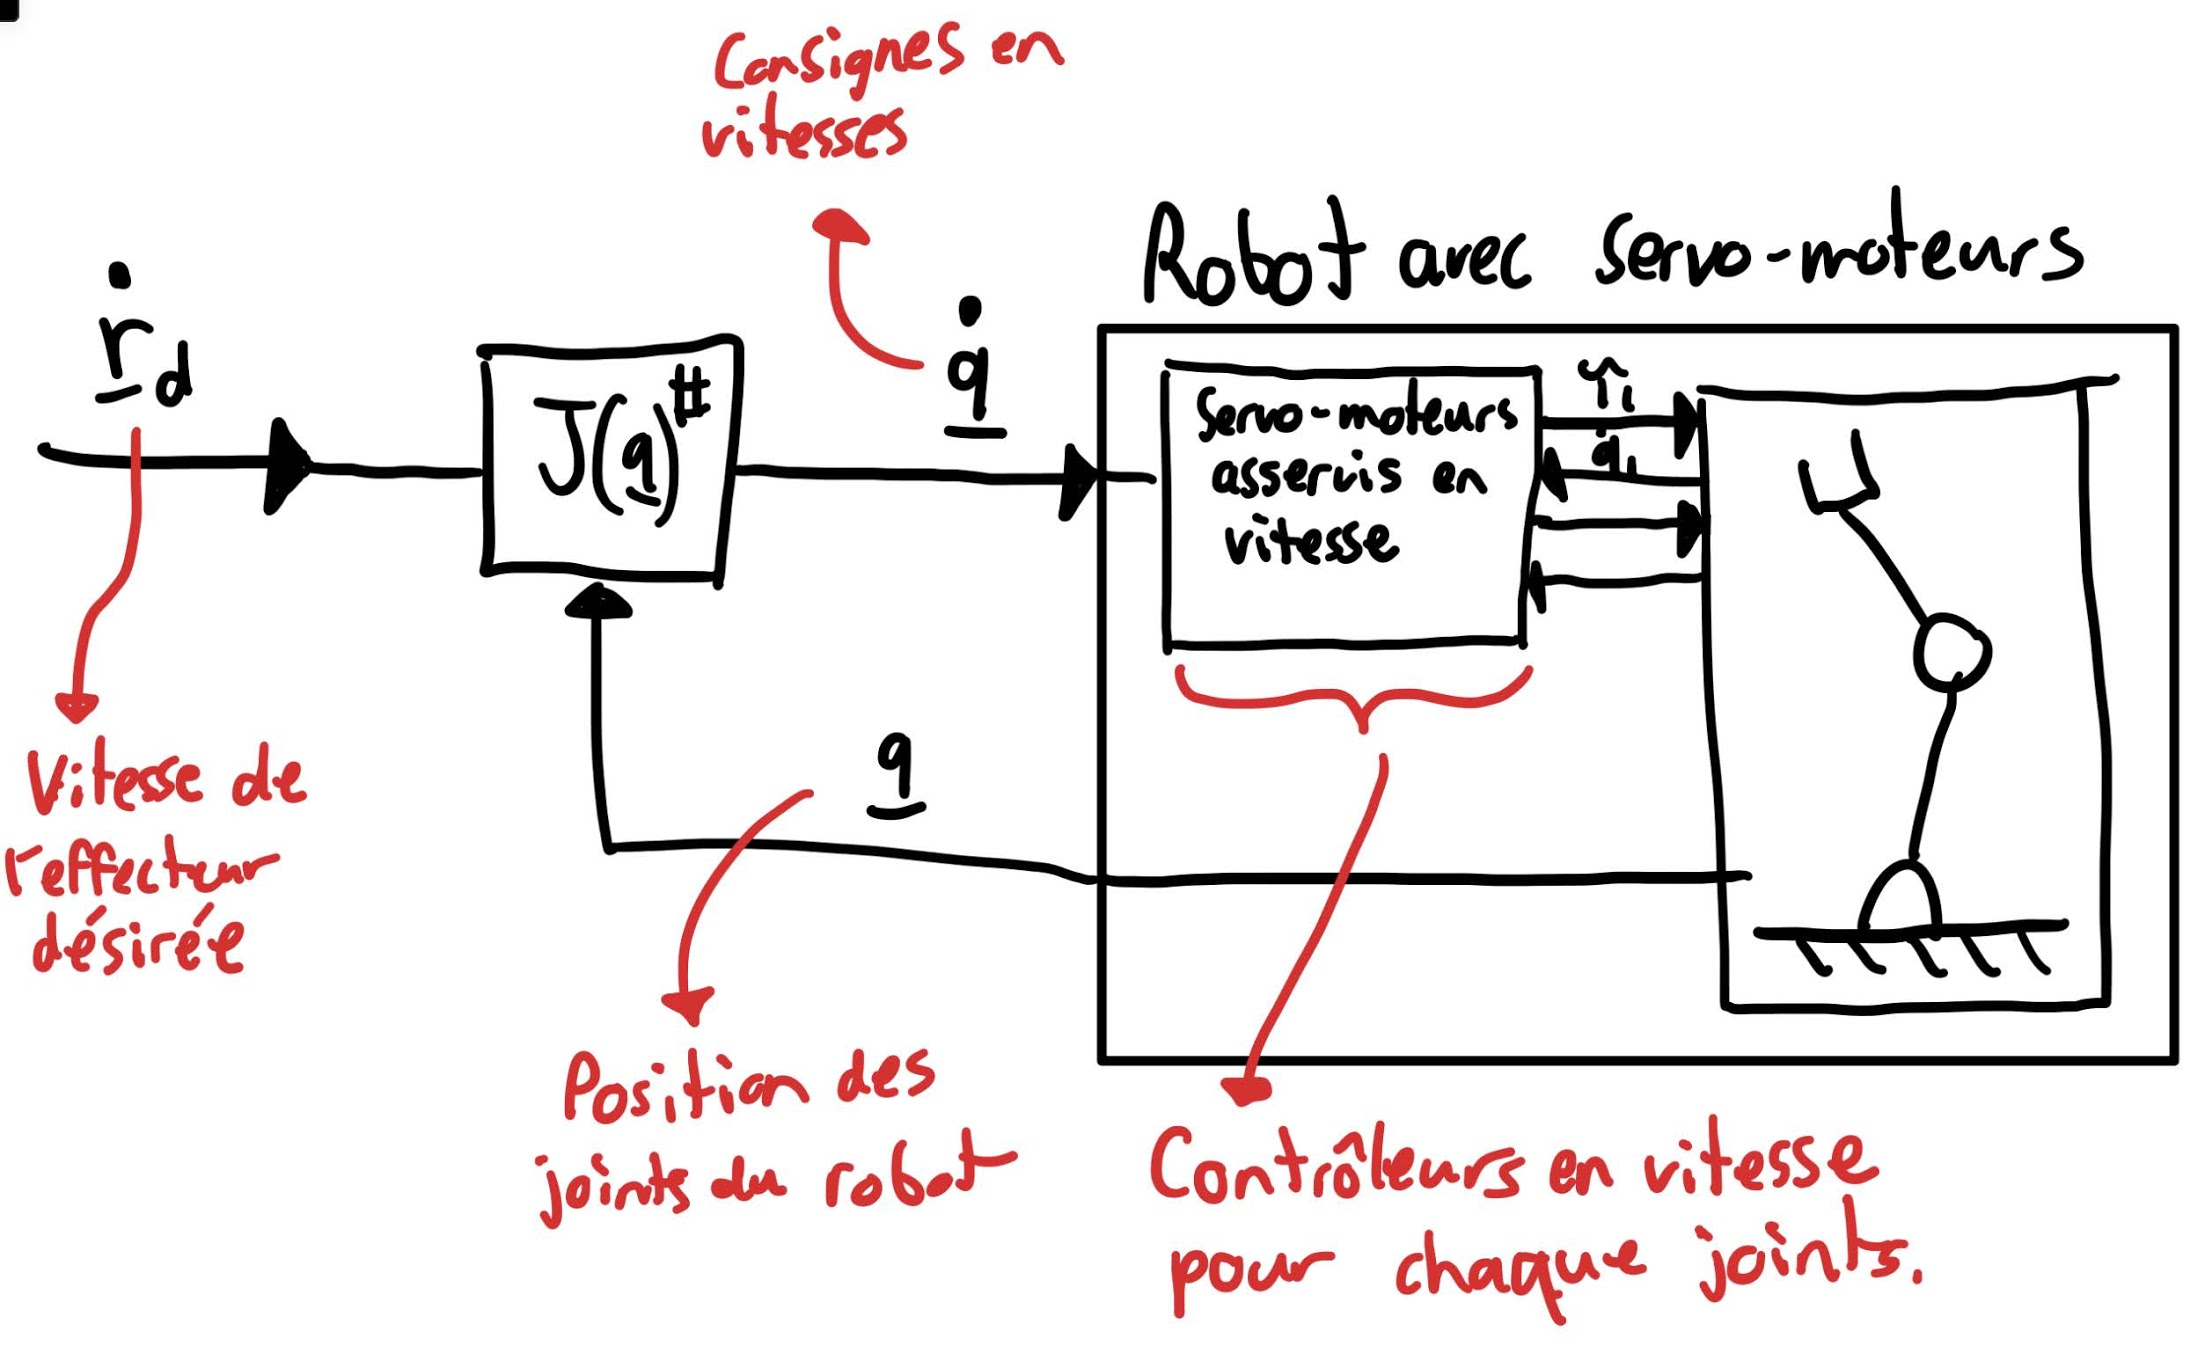
\includegraphics[width=0.7\textwidth]{fig/robotspeedcontrol.jpg}
	\caption{Commande de la vitesse de l'effecteur d'un robot : schéma bloc}
	\label{fig:robotspeedcontrol}
\end{figure}
%%%%%%%%%%%%%%%%%%%%%%%%%%%%%%%%

Si le nombre de joints $n$ est égale au nombre de DDL de l'espace de la tâche $m$, alors la matrice Jacobienne est carrée et peut être inversée (sauf sur les singularités). Si le nombre de joint $n$ est supérieur au nombre de DDL de l'espace de la tâche $m$, alors on peut utiliser une matrice pseudo-inverse droite $J^{\#} = J^T (J J^T)^{-1}$ (voir section \ref{sec:pseudoinverse}). La loi de commande en équation peut donc être exprimée comme:
%%%%%%%%%%%%%%%%%%
\begin{align}
\dot{\col{q}} = \left\{ \begin{array}{c}
 J(\col{q})^{-1} \dot{\col{r}_d}   \quad\quad \text{if $n=m$}
 \\ \\
 J(\col{q})^{\#} \, \dot{\col{r}_d}   \quad\quad \text{if $n>m$}
\end{array}
\right.
\end{align}
%%%%%%%%%%%%%%%%%

En substituant la loi de commande dans la relation de cinématique différentielle, on confirme que la vitesse de l'effecteur sera exactement la vitesse désirée:
%%%%%%%%%%%%%%%%%%
\begin{align}
\dot{\col{r}} &= J(\col{q}) \, \dot{\col{q}} \\
\dot{\col{r}} &= J(\col{q}) \, J(\col{q})^{\#} \, \dot{\col{r}_d} \\
\dot{\col{r}} &= J J^T (J J^T)^{-1} \, \dot{\col{r}_d} \\
\dot{\col{r}} &=  \col{\dot{r}_d} 
\end{align}
%%%%%%%%%%%%%%%%%
sous les hypothèses que: 1) le Jacobien utilisé par le contrôleur est exacte, 2) le Jacobien est inversible (i.e. le robot n'est pas sur une singularité) et 3) la vitesse des joints est parfaitement asservis par les boucles bas-niveaux. 




%%%%%%%%%%%%%%%%%%%%%%%%%%%%%%%%%%%%%%%%%%%%%%%%%%%%%%
\newpage
\section{Commande en position de l'effecteur}
\label{sec:positioncontrol}
%%%%%%%%%%%%%%%%%%%%%%%%%%%%%%%%%%%%%%%%%%%%%%%%%%%%%%

Pour commander la position de l'effecteur d'un robot, tenter de trouver une solution directement au problème de cinématique inverse (voir section \ref{sec:invkin}) n'est généralement pas la méthode la plus appropriée car la cinématique directe des manipulateurs est hautement non-linéaire. La méthode ici présentée utilise plutôt la méthode de commande en vitesse de l'effecteur (section \ref{sec:speedcontrol}) pour indirectement résoudre la cinématique inverse du robot. Le principe ce résume au fait que pour contrôler la position de l'effecteur, il suffit de diriger le vecteur vitesse de l'effecteur vers la position cible. La méthode est illustrée graphiquement à la Figure \ref{fig:robotspeedcontrolgeo}: 1) Un vecteur d'erreur $\col{r}_e$ est calculé en comparant la position désirée $\col{r}_d$ à la position actuelle $\col{r}$. 2) Le vecteur d'erreur $\col{r}_e$ est multiplié par un paramètre scalaire $\lambda$ pour déterminer la vitesse cible instantanée pour l'effecteur notée $\dot{\col{r}}_r$, qui pointe en direction de la cible. 3) L'inverse du Jacobien est utilisé pour convertir la vitesse instantanée désirée de l'effecteur en consignes de vitesse pour les joints. 
%%%%%%%%%%%%%%%%%%%%%%%%%%%%%%%%
\begin{figure}[H]
	\centering
		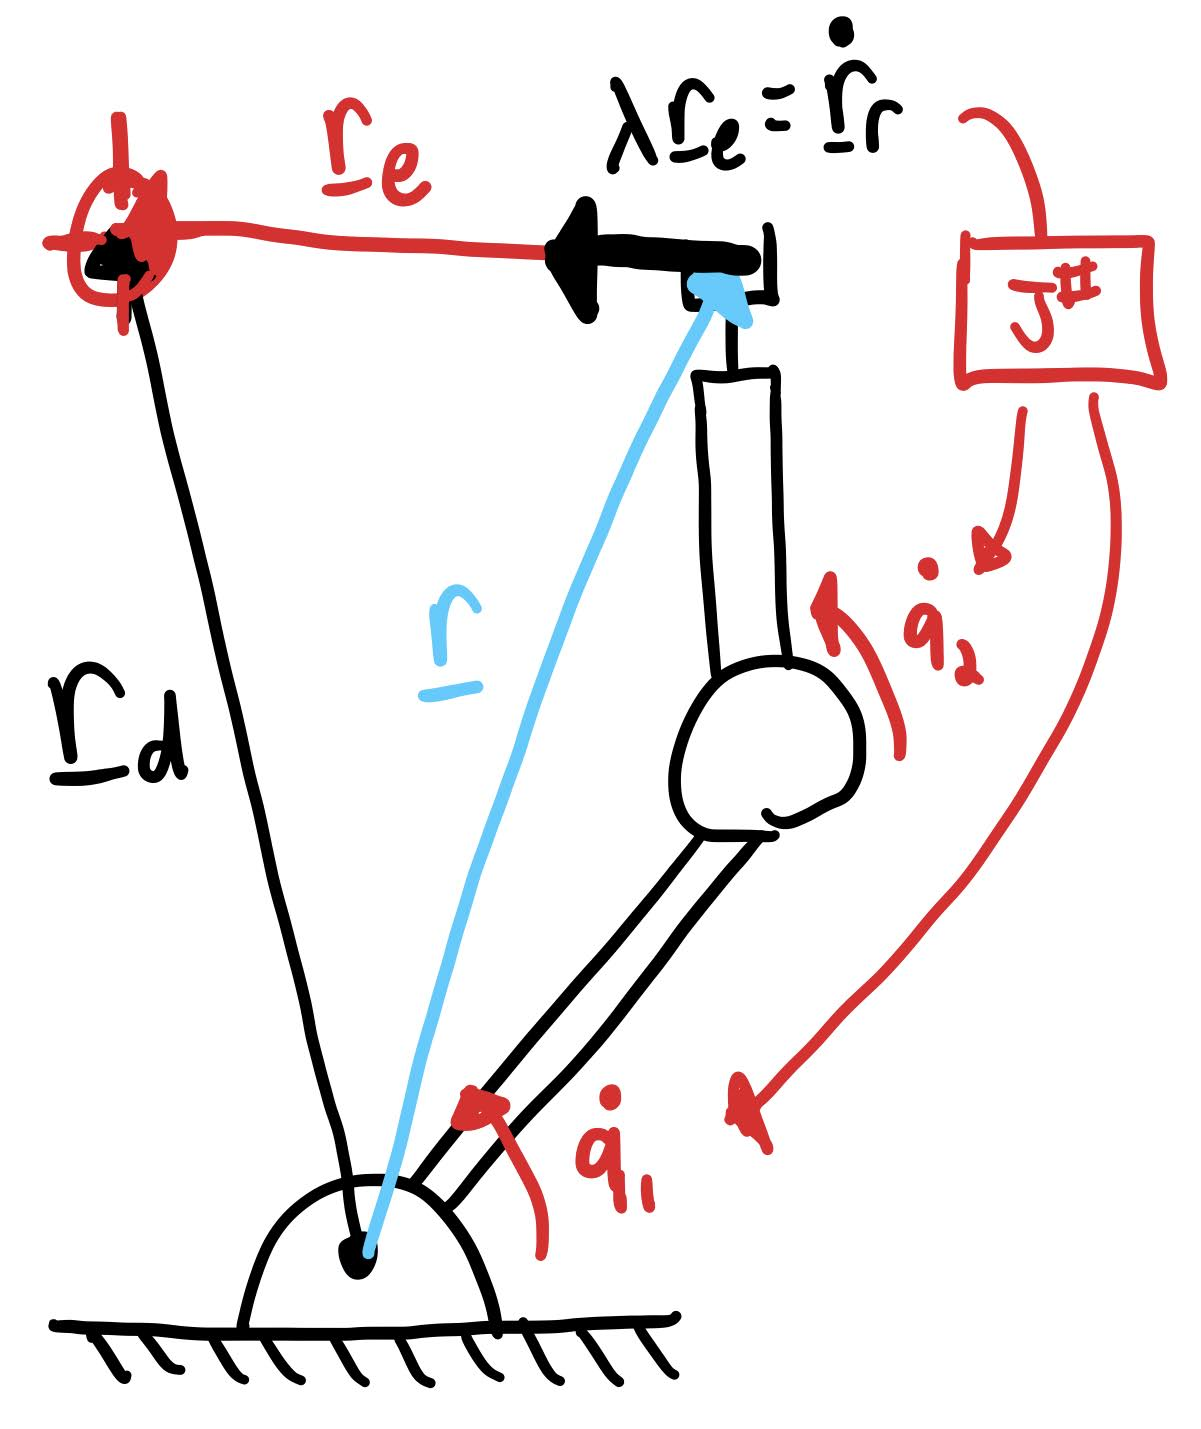
\includegraphics[width=0.35\textwidth]{fig/robotspeedcontrolgeo.jpg}
	\caption{Commande de la trajectoire de l'effecteur d'un robot : interprétation géométrique}
	\label{fig:robotspeedcontrolgeo}
\end{figure}
%%%%%%%%%%%%%%%%%%%%%%%%%%%%%%%%

\video{Commande du mouvement de l'effecteur d'un robot manipulateur}{https://youtu.be/Qo60ySYaMqg}


Formellement, la loi de commande est exprimée par l'expression mathématique:
%%%%%%%%%%%%%%%%%%
\begin{align}
\dot{\col{q}} = \left\{ \begin{array}{c}
 J(\col{q})^{-1} \lambda 
 \underbrace{ \left( \col{r}_d  - \underbrace{f(\col{q})}_{\col{r}}  \right) }_{\col{r}_e} 
 \quad\quad \text{if $n=m$}
 \\ \\
 J(\col{q})^{\#} \, \lambda  \underbrace{ \left( \col{r}_d  - \underbrace{f(\col{q})}_{\col{r}}  \right) }_{\col{r}_e}    \quad\quad \text{if $n>m$}
\end{array}
\right.
\end{align}
%%%%%%%%%%%%%%%%%
ou $\lambda$ est un paramètre scalaire de gain du contrôleur, $J$ est le Jacobien, la matrice $n \times m$, qui relie l'espace des joints à l'espace de la tâche du manipulateur, et $f(\col{q})$ la fonction de cinématique directe du manipulateur. La Figure \ref{fig:robotspeedcontrolpos} illustre cette méthode de commande sous la forme d'un schéma bloc. 
%%%%%%%%%%%%%%%%%%%%%%%%%%%%%%%%
\begin{figure}[H]
	\centering
		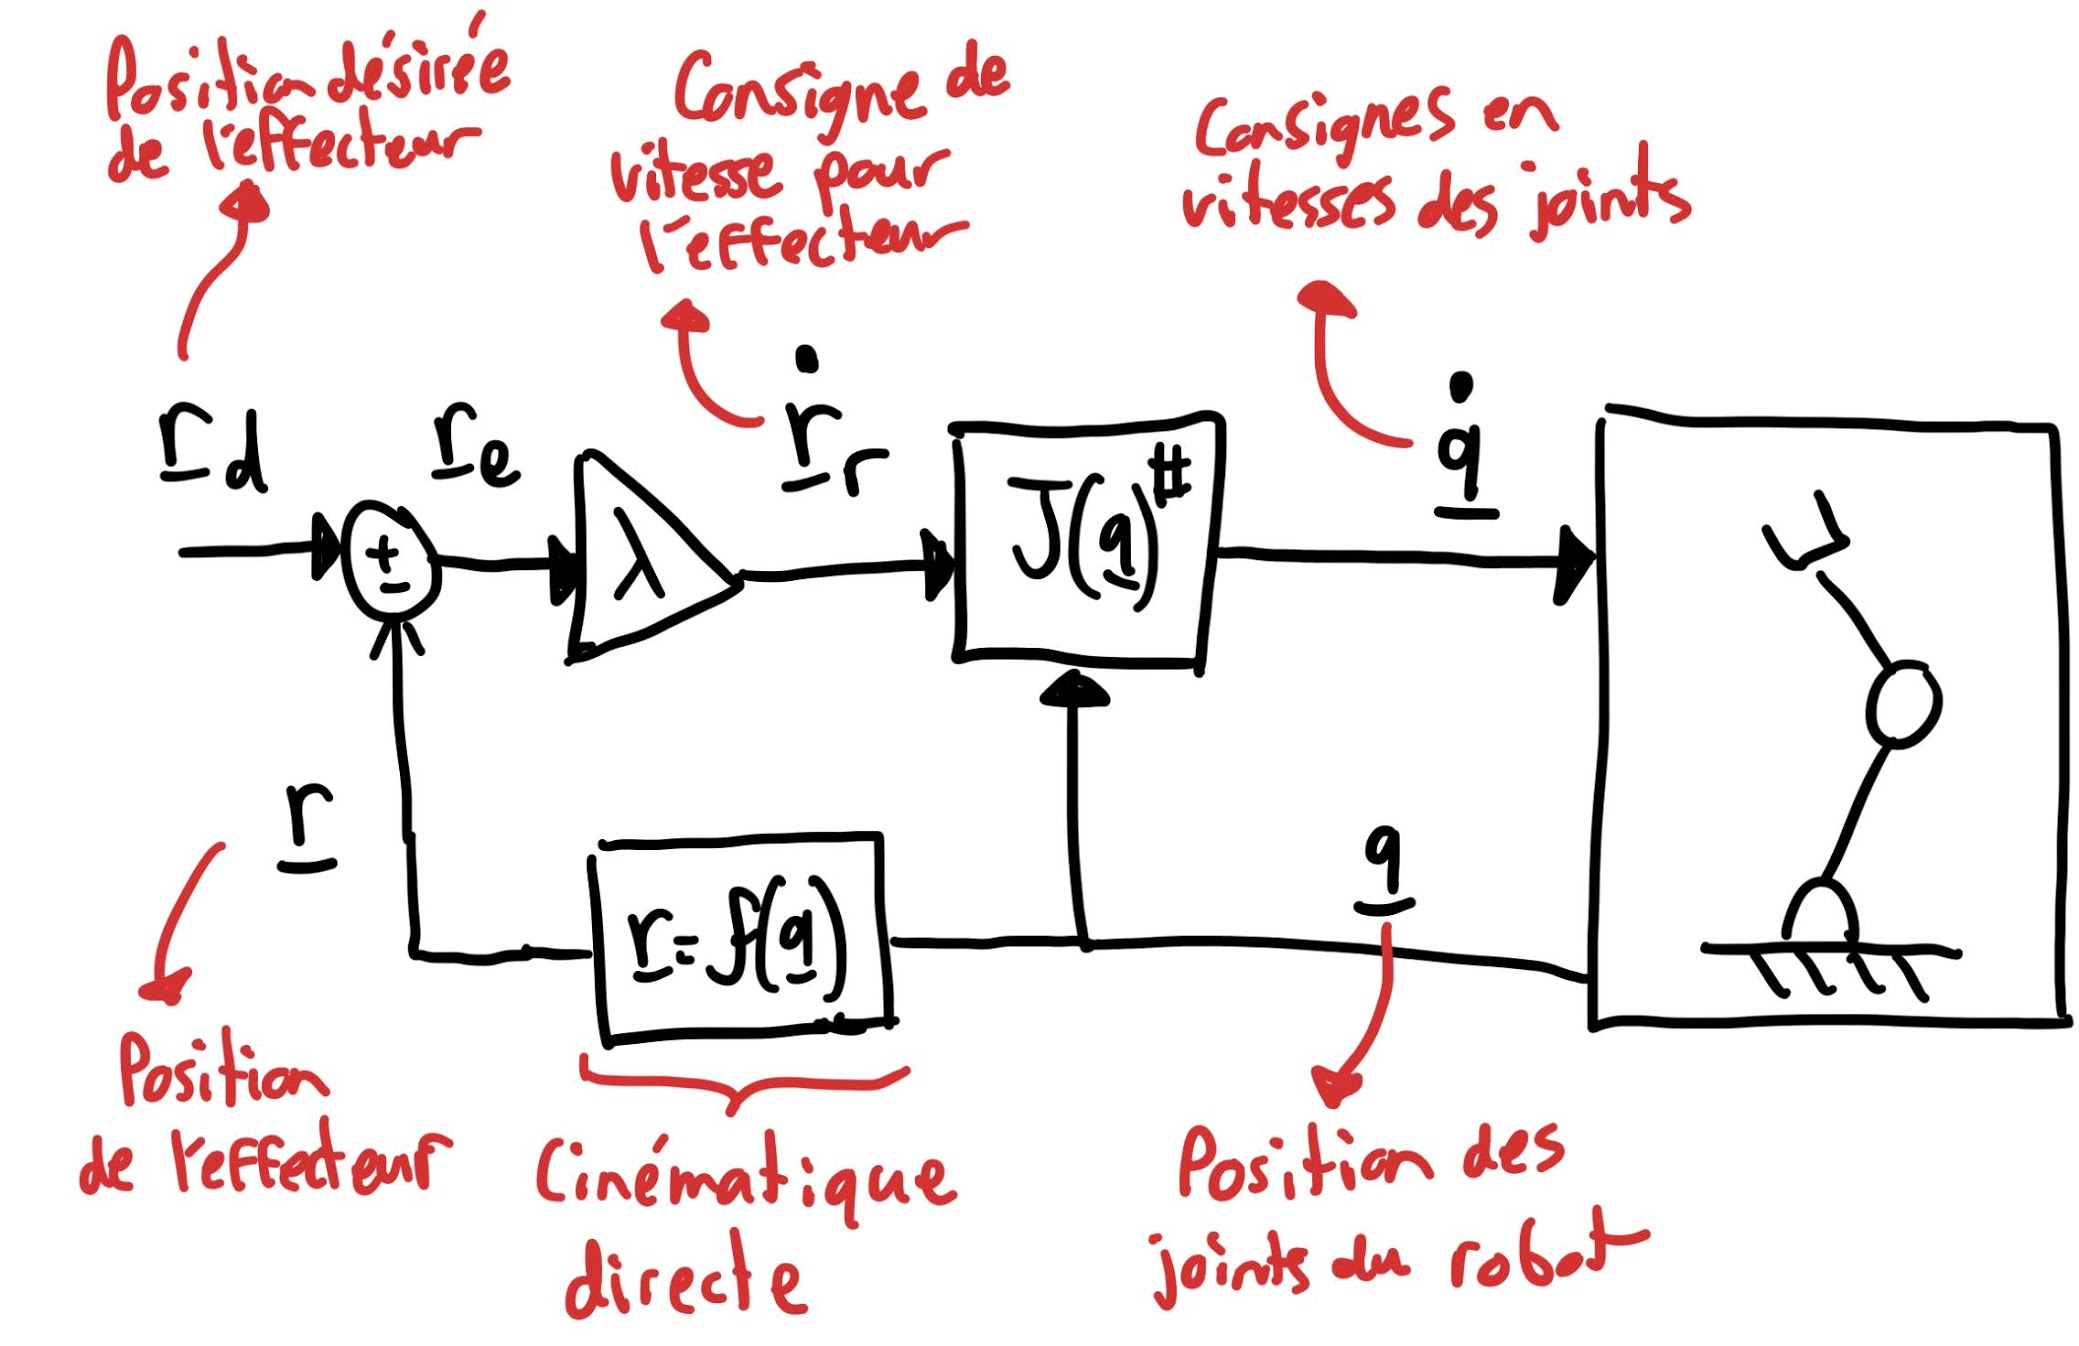
\includegraphics[width=0.7\textwidth]{fig/robotspeedcontrolpos.jpg}
	\caption{Commande de la position de l'effecteur d'un robot : schéma bloc}
	\label{fig:robotspeedcontrolpos}
\end{figure}
%%%%%%%%%%%%%%%%%%%%%%%%%%%%%%%%




\colab{Commande d'un manipulateur en position}{https://colab.research.google.com/drive/1M3O_nD8iLbRSvZzyUpBn0Mo8KUclrG26?usp=sharing}





%%%%%%%%%%%%%%%%%%%%%%%%%%%%%%%%%%%%%%%%%%%%%%%%%%%%%%%%%%%%%%%%
\subsection{Suivi de trajectoire}
\label{sec:trajcontrol}

Lorsque le robot doit suivre une position cible de l'effecteur qui varie dans le temps, il est préférable de calculer la dérivée temporelle de la trajectoire et d'utiliser cette information directement dans la loi de commande comme indiqué dans l'équation suivante:
%%%%%%%%%%%%%%%%%%
\begin{align}
\dot{\col{q}} = \left\{ \begin{array}{c}
 J(\col{q})^{-1} \left[ \dot{\col{r}_d} + \lambda \left( \col{r}_d  - \underbrace{f(\col{q})}_{\col{r}} \right) \right] \quad\quad \text{if $n=m$}
 \\ \\
 J(\col{q})^{\#} \, \left[ \dot{\col{r}_d} + \lambda \left( \col{r}_d  - \underbrace{f(\col{q})}_{\col{r}} \right) \right]   \quad\quad \text{if $n>m$}
\end{array}
\right.
\end{align}
%%%%%%%%%%%%%%%%%
En terme de schéma bloc, la vitesse de la trajectoire doit être utilisée comme illustré à la Figure \ref{fig:robotspeedcontroltraj}, ce qu'on appel un \textit{feedforward} en anglais, pour garantir la convergence sur la trajectoire.
%%%%%%%%%%%%%%%%%%%%%%%%%%%%%%%%
\begin{figure}[H]
	\centering
		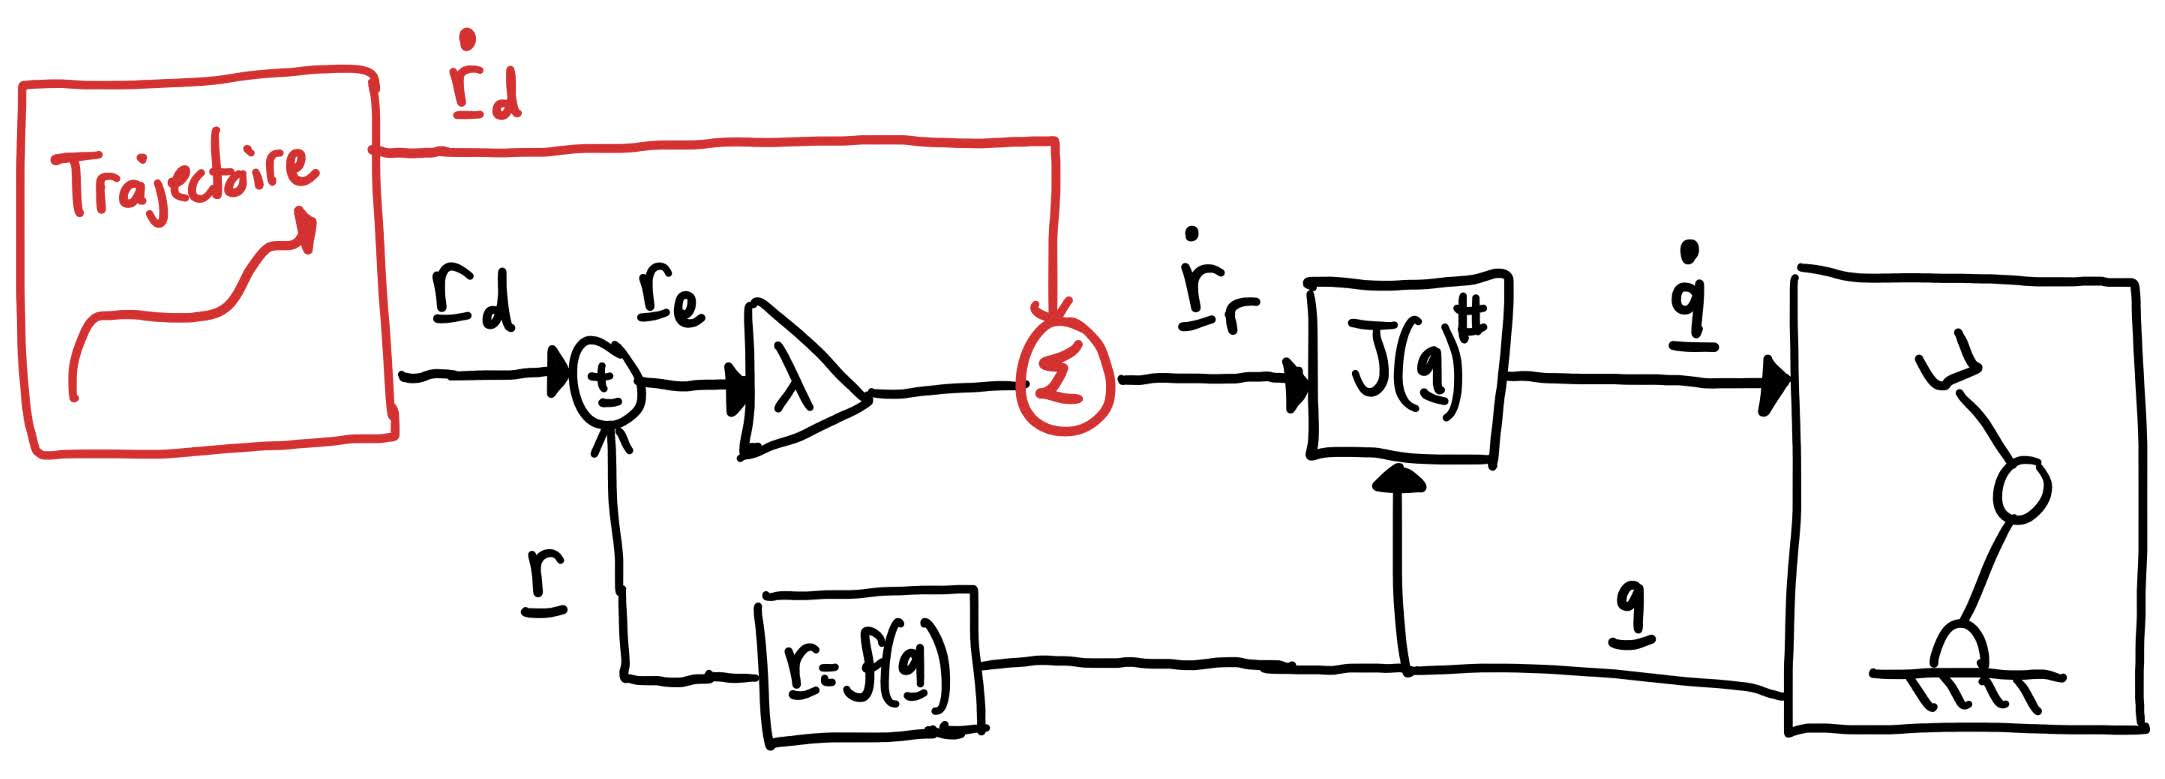
\includegraphics[width=0.95\textwidth]{fig/robotspeedcontroltraj.jpg}
	\caption{Commande de la trajectoire de l'effecteur d'un robot : schéma bloc}
	\label{fig:robotspeedcontroltraj}
\end{figure}
%%%%%%%%%%%%%%%%%%%%%%%%%%%%%%%%


\subsection{Convergence}

Les méthodes de commande en position de l'effecteur convergent sous certaines conditions, i.e. l'erreur (sur la position de l'effecteur) converge vers zéro lorsque le temps tend vers l'infini:
%%%%%%%%%%%%%%%%%%
\begin{align}
\lim_{t \rightarrow \infty } \col{r}_e(t) = 0 
\end{align}
%%%%%%%%%%%%%%%%%

\begin{proof}
L'erreur est une fonction de la position désirée et de la positon réelle du robot:
%%%%%%%%%%%%%%%%%%
\begin{align}
\col{r}_e = \col{r}_d - \col{r}
\end{align}
%%%%%%%%%%%%%%%%%
Si on dérive cette équation dans le temps, on obtient une relation différentielle. On peut alors substituer le modèle de cinématique différentiel et les lois de commandes pour obtenir:
%%%%%%%%%%%%%%%%%%
\begin{align}
\dot{\col{r}}_e  &= \dot{\col{r}}_d - \dot{\col{r}} \\
\dot{\col{r}}_e  &= \dot{\col{r}}_d - J(\col{q}) \dot{\col{q}} \\
\dot{\col{r}}_e  &= \dot{\col{r}}_d - \underbrace{J(\col{q}) J(\col{q})^{\#} }_{1} \dot{\col{r}}_r \\
\dot{\col{r}}_e  &= \dot{\col{r}}_d - \underbrace{J(\col{q}) J(\col{q})^{\#} }_{1}  \left( \dot{\col{r}}_d + \lambda \, \col{r}_e \right) \\
\dot{\col{r}}_e  &= - \lambda \, \col{r}_e  
\end{align}
%%%%%%%%%%%%%%%%
La dynamique de l'erreur est une équation différentielle d'ordre 1. Si la constante de temps est positive $\lambda>0$ (ici directement déterminée par le gain de notre contrôleur), l'erreur converge exponentiellement vers zéro:
%%%%%%%%%%%%%%%%%%
\begin{align}
\dot{\col{r}}_e = - \lambda \, \col{r}_e 
\quad\quad \Rightarrow \quad\quad 
\col{r}_e(t) = \col{r}_e(t=0) \, e^{- \lambda t} 
\quad\quad \Rightarrow \quad\quad 
\col{r}_e(t=\infty) = 0
\end{align}
%%%%%%%%%%%%%%%%%
\end{proof}
Notez ici que cette analyse assume un contrôle parfait et instantané de la vitesse des moteurs. Une autre limite est que la convergence cesse si le robot passe sur une singularité, i.e. mathématiquement l'inverse (ou pseudo-inverse) du Jacobien n'excisera pas. Finalement, comme démontré dans la démarche, pour garantir la convergence exponentielle sur une trajectoire (position cible qui varie dans le temps), le terme de \textit{feedforward} illustré à la Figure \ref{fig:robotspeedcontroltraj} est nécessaire.




%%%%%%%%%%%%%%%%%%%%%%%%%%%%%%%%%%%%%%%%%%%%%%%%%%%%%%%%%%%
\newpage
\subsection{Utilisation de l'espace nul pour un objectif secondaire}

Comme il a été vu à la section \ref{sec:invdiffkinredondant}, lorsque le nombre de DDL du robot $n = dim(\col{q})$  est supérieur à celui de l'espace de la tâche qu'on désire contrôler $m = dim(\col{r})$, il y a plusieurs solutions $\col{\dot{q}}$ pour lesquels la vitesse cible pour l'effecteur est parfaitement atteinte. Lorsque la consigne de vitesse de l'effecteur $\col{\dot{r}}_r$ est fixée par la loi de commande qui la fait converger vers $\col{r}_d$,  l'ensemble des solutions pour $\dot{\col{q}}$ peuvent être décrite par l'équation suivante:
%%%%%%%%%%%%%%%%%%
\begin{align}
\dot{\col{q}} = J^{\#} \, 
\underbrace{
\left[ \dot{\col{r}_d} + \lambda \left( \col{r}_d  - \underbrace{f(\col{q})}_{\col{r}}  \right)\right] 
}_{\col{\dot{r}}_r}
+ \left[ I - J^{\#}J  \right] \col{v}
\end{align}
%%%%%%%%%%%%%%%%%
où le vecteur-colonne $\col{v}$ contient les variables libres. On peut donc considérer le vecteur $\col{v}$ comme une entrée de contrôle secondaire, qu'il est possible d'utiliser pour faire autre chose avec le robot sans affecter la convergence de l'effecteur. Par exemple, les bras humains: on peut les utiliser pour attraper un objet avec notre main (objectif principal), tout en utilisant notre bras pour tenir un cahier contre notre corps (objectif secondaire). On peut aussi utiliser l'espace nul pour tenter de garder la configuration du robot le plus loin possible des configurations singulières. La Figure \ref{fig:nullspacecontrol} illustre graphiquement l'effet de divers options de vecteur $\col{v}$ sur les mouvements internes des joints d'un robot manipulateur redondant. 

%%%%%%%%%%%%%%%%%%%%%%%%%%%%%%%%
\begin{figure}[H]
	\centering
		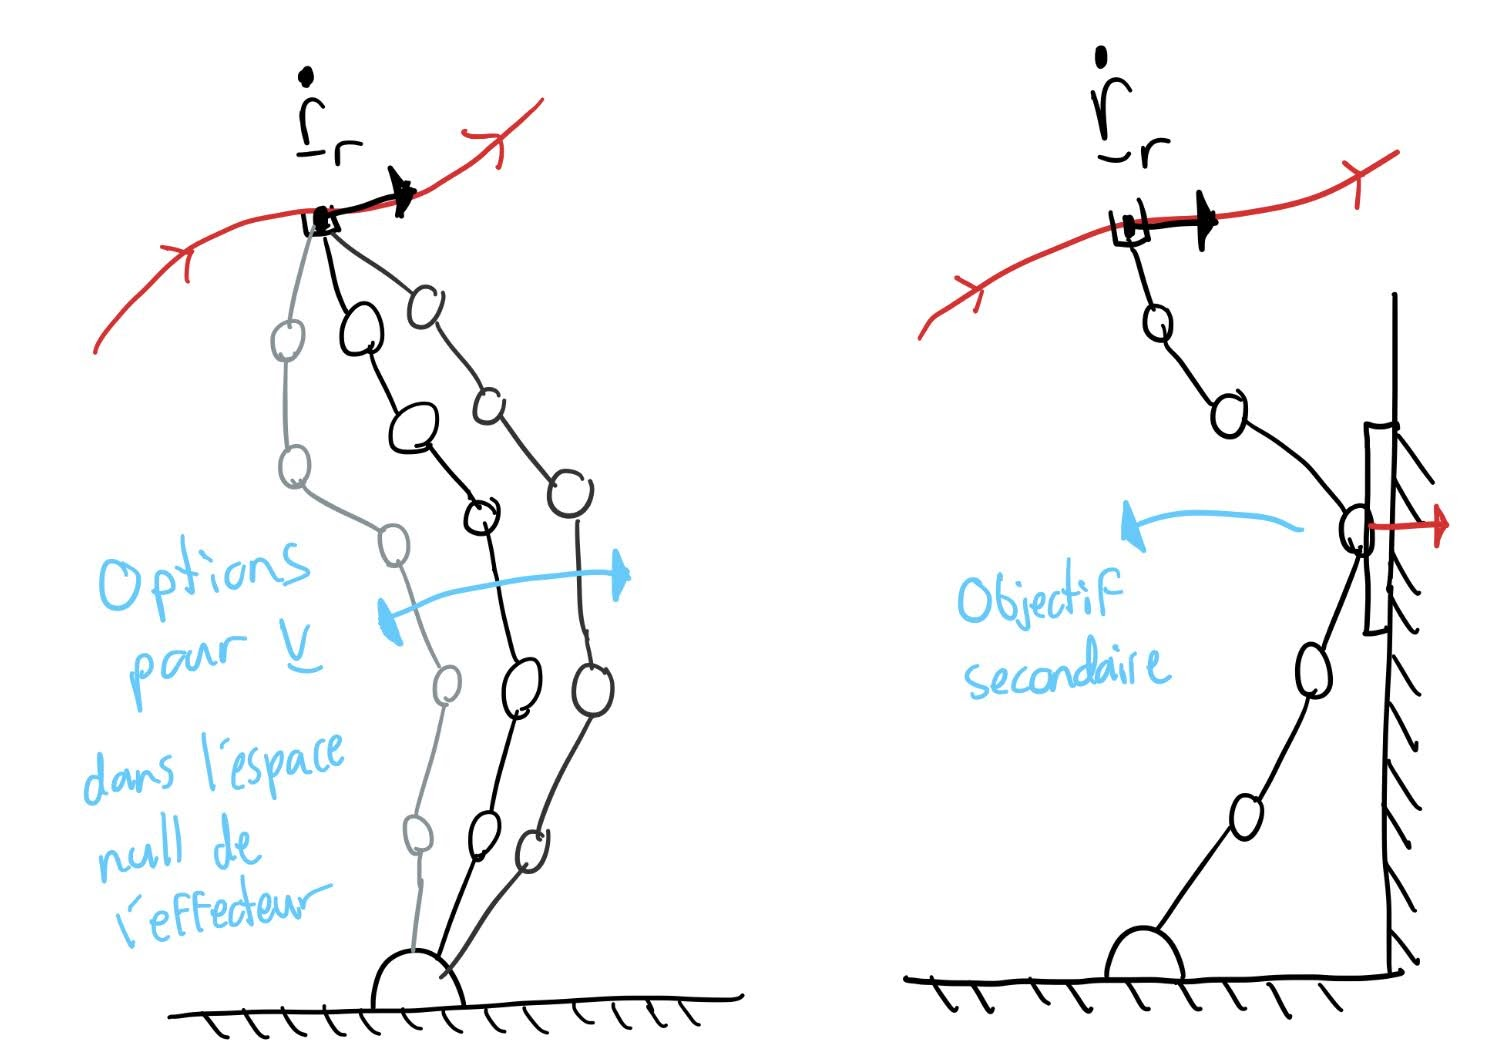
\includegraphics[width=0.70\textwidth]{fig/nullspacecontrol.jpg}
	\caption{Utilisation de l'espace nul d'un robot redondant pour effectuer un objectif secondaire}
	\label{fig:nullspacecontrol}
\end{figure}
%%%%%%%%%%%%%%%%%%%%%%%%%%%%%%%%

\video{Commande de l'effecteur d'un robot redondant}{https://youtu.be/R0T4shGPBKo}

De façon général, on peut formuler l'objectif secondaire comme une fonction potentielle scalaire $G$ qui dépend de la configuration (un scalaire qui est le plus grand possible le plus on est loin de l'objectif). La commande secondaire $\col{v}$ peut alors être déterminée par le gradient de cette fonction évalué à la configuration actuelle du robot:
%%%%%%%%%%%%%%%%%%
\begin{align}
G( \col{q} ) \; \Rightarrow \; \col{v} = \frac{\partial G }{\partial \col{q} }
\end{align}
%%%%%%%%%%%%%%%%%

Si l'objectif secondaire est une position cible $\col{q}_d$ dans l'espace des joints. La fonction objectif $G$ pourrait être la norme de l'erreur, et on obtiendrait:
%%%%%%%%%%%%%%%%%%
\begin{align}
G( \col{q} ) &= - \frac{1}{2} \lambda \col{q}_e^T \col{q}_e
\quad \text{avec: } \; \col{q}_e = \col{q}_d - \col{q} \\
\col{v} &= \frac{\partial G }{\partial \col{q} } = \lambda \huge( \col{q}_d - \col{q} \huge)
\end{align}
%%%%%%%%%%%%%%%%%
où $\lambda$ est un paramètre de gain de convergence pour cette boucle de commande secondaire avec une cible de configuration $\col{q}_d$ dans l'espace des joints. Notez que la boucle principale a toujours la priorité absolue avec cette formulation, la convergence de l'objectif principal est garantie mais pas celle de l'objectif secondaire. 

\colab{Espace nul d'un robot redondant}{https://colab.research.google.com/drive/16ACenFOLOHVNeReqJTbkATAB3281iVbp?usp=sharing}


%%%%%%%%%%%%%%%%%%%%%%%%%%%%%%%%%%%%%%%%%%%%%%%%%%%%%%%%%%%
\subsection{Formulation avec régulation de la norme du vecteur vitesse}

Dans certaines situation, par exemple lorsque le robot passe proche d'une singularité, les lois de commande présentées dans les sections précédentes peuvent demander des très grande vitesses irréalistes aux joints. Plutôt que d'inverser directement la matrice Jacobienne, il est possible de plutôt trouver une solution au système d'équation suivant qui pénalise aussi la norme du vecteur $\col{\dot{q}}$:
%%%%%%%%%%%%%%%%%%%%%%%%%%%%%%%%%%%
\begin{align}
\left[ \begin{array}{c}  \\ \dot{\col{r}}_r \\ \\ \col{0} \\ \\ 
\end{array} \right]_{(m+n) \times 1}
&= 
\left[ \begin{array}{c c c} 
&&\\
& J(\col{q}) &\\
&&\\
&\lambda I &\\
&&
\end{array} \right]_{(m + n)  \times n}
\left[ \begin{array}{c} 
\\ \dot{\col{q}} \\ \\
\end{array} \right]_{n \times 1}
\end{align} 
%%%%%%%%%%%%%%%%%%%%%%%%%%%%%%%%%%%
où $\lambda$ est un paramètre de poids sur la pénalité d'utiliser des grandes vitesses de joints. Ce système a donc $m+n$ équations et $n$ variables, il est donc sur-contraint. Une méthode standard est d'utiliser la solution des moindres-carrés (voir section \ref{sec:moindrecarre}) pour trouver une solution non-exacte pour $\dot{\col{q}}$ qui minimise la norme de l'erreur au carré, ce qui correspond ici à minimiser:
%%%%%%%%%%%%%%%%%%%%%%%%%%%%%%%%%%%
\begin{align}
\| \col{e} \|^2 = \| \col{\dot{r}}_r - J \col{\dot{q}}   \|^2 + \lambda^2 \| \col{\dot{q}} \|^2
\end{align} 
%%%%%%%%%%%%%%%%%%%%%%%%%%%%%%%%%%%
La solution des moindres carrés a une solution explicite qui correspond à 
%%%%%%%%%%%%%%%%%%%%%%%%%%%%%%%%%%%
\begin{align}
\col{\hat{\dot{q}}} &= \operatornamewithlimits{argmin}\limits_{\col{\dot{q}}} \| \col{e} \|^2 \\
\col{\hat{\dot{q}}} &= \huge( J^T J + \lambda^2 I \huge)^{-1} J^T  \col{\dot{r}}_r 
\end{align} 
%%%%%%%%%%%%%%%%%%%%%%%%%%%%%%%%%%%
La convergence de cette méthode n'est toutefois pas garantie, le robot peut dériver de la trajectoire désirée surtout si $\lambda$ est trop grand. Une méthode pour palier à ce problème est d'ajuster dynamiquement $\lambda$ pour lui assigner de grandes valeurs seulement proche des configurations problématiques, i.e. proche des singularités. Dans la littérature, la méthode présentée dans cette section est appelée \textit{damped least-square}.

\video{Commande en position avec régulation de vitesse}{https://youtu.be/n3G-O7cpQTQ}


%%%%%%%%%%%%%%%%%%%%%%%%%%%%%%%%%%%%%%%%%%%%%%%%%%%%%%
\newpage
\section{Commande en force de l'effecteur}
\label{sec:forcecontrol}
%%%%%%%%%%%%%%%%%%%%%%%%%%%%%%%%%%%%%%%%%%%%%%%%%%%%%%

Pour certaines tâches, ce n'est pas la position de l'outil que l'on désire contrôler, mais plutôt la force qu'il applique sur l'environnement. Si un systèmes robotisé a des actionneurs qui sont contrôlable en force ou couple, il suffit d'une transformation géométrique avec le Jacobien pour calculer les consignes en force des actionneurs basé sur une force désirée à l'effecteur, comme illustré à la Figure \ref{fig:forcecontroleffectorgeo}. 
%%%%%%%%%%%%%%%%%%%%%%%%%%%%%%%%
\begin{figure}[H]
	\centering
		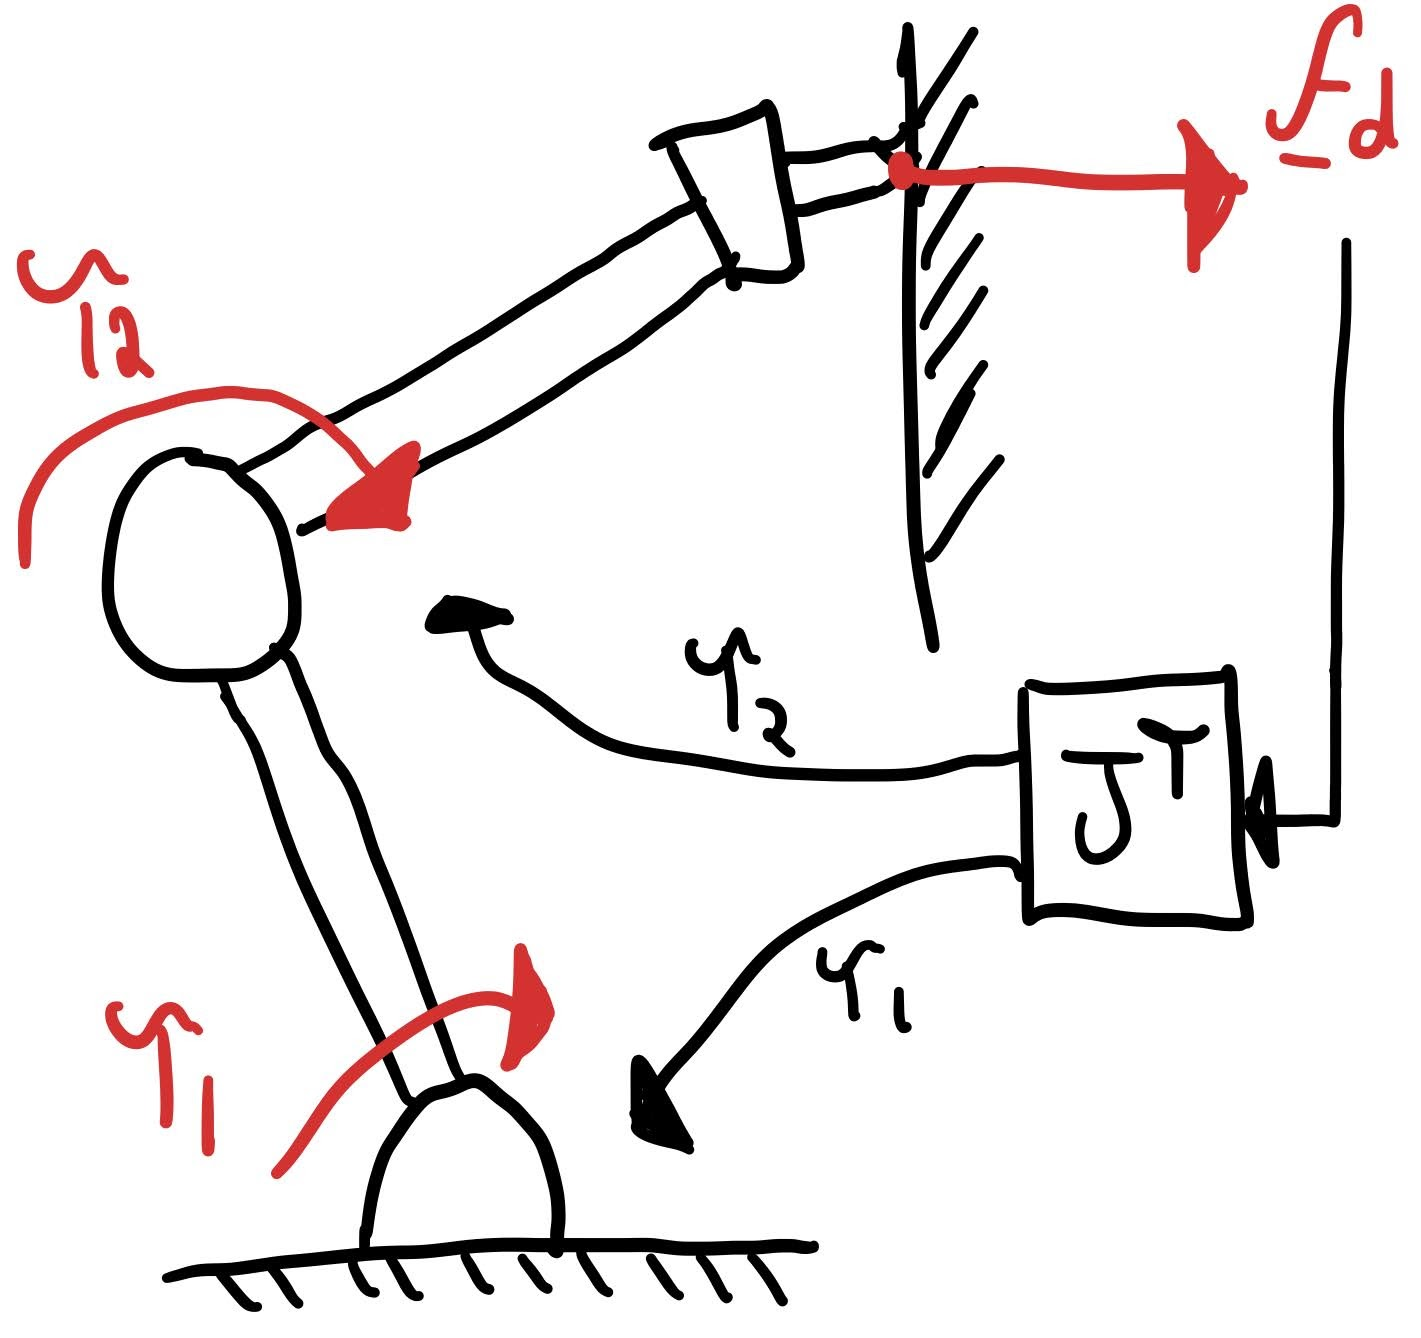
\includegraphics[width=0.35\textwidth]{fig/forcecontroleffectorgeo.jpg}
	\caption{Commande en force de l'effecteur d'un robot : interprétation géométrique}
	\label{fig:forcecontroleffectorgeo}
\end{figure}
%%%%%%%%%%%%%%%%%%%%%%%%%%%%%%%%

\video{Commande en force d'un robot manipulateur}{https://youtu.be/mDQInbWXcj4}

La Figure \ref{fig:forcecontroleffectorbloc} montre cette méthode de commande avec un schéma bloc. À l'exception du calcul du Jacobien qui nécessite de connaître la position des joints actuelle, la méthode peut être peut être considérée comme une boucle ouverte.  Par exemple dans le cas des robots à entraînement direct, i.e. utilisant des gros moteurs électrique qui n'ont pas de ratio de réduction, il suffit de traduire la force désirée en couples moteurs à l'aide du Jacobien et ensuite de traduire les couples moteurs en consigne de courant des les moteurs en divisant par la constante des moteurs. Selon le type d'actionneur, des boucles de rétroaction en force à bas niveau peuvent être utilisées, par exemple un asservissement de la pression dans un actionneur pneumatique. La loi de commande présentée ici spécifie les consignes en force pour les actionneurs.
%%%%%%%%%%%%%%%%%%%%%%%%%%%%%%%%
\begin{figure}[H]
	\centering
		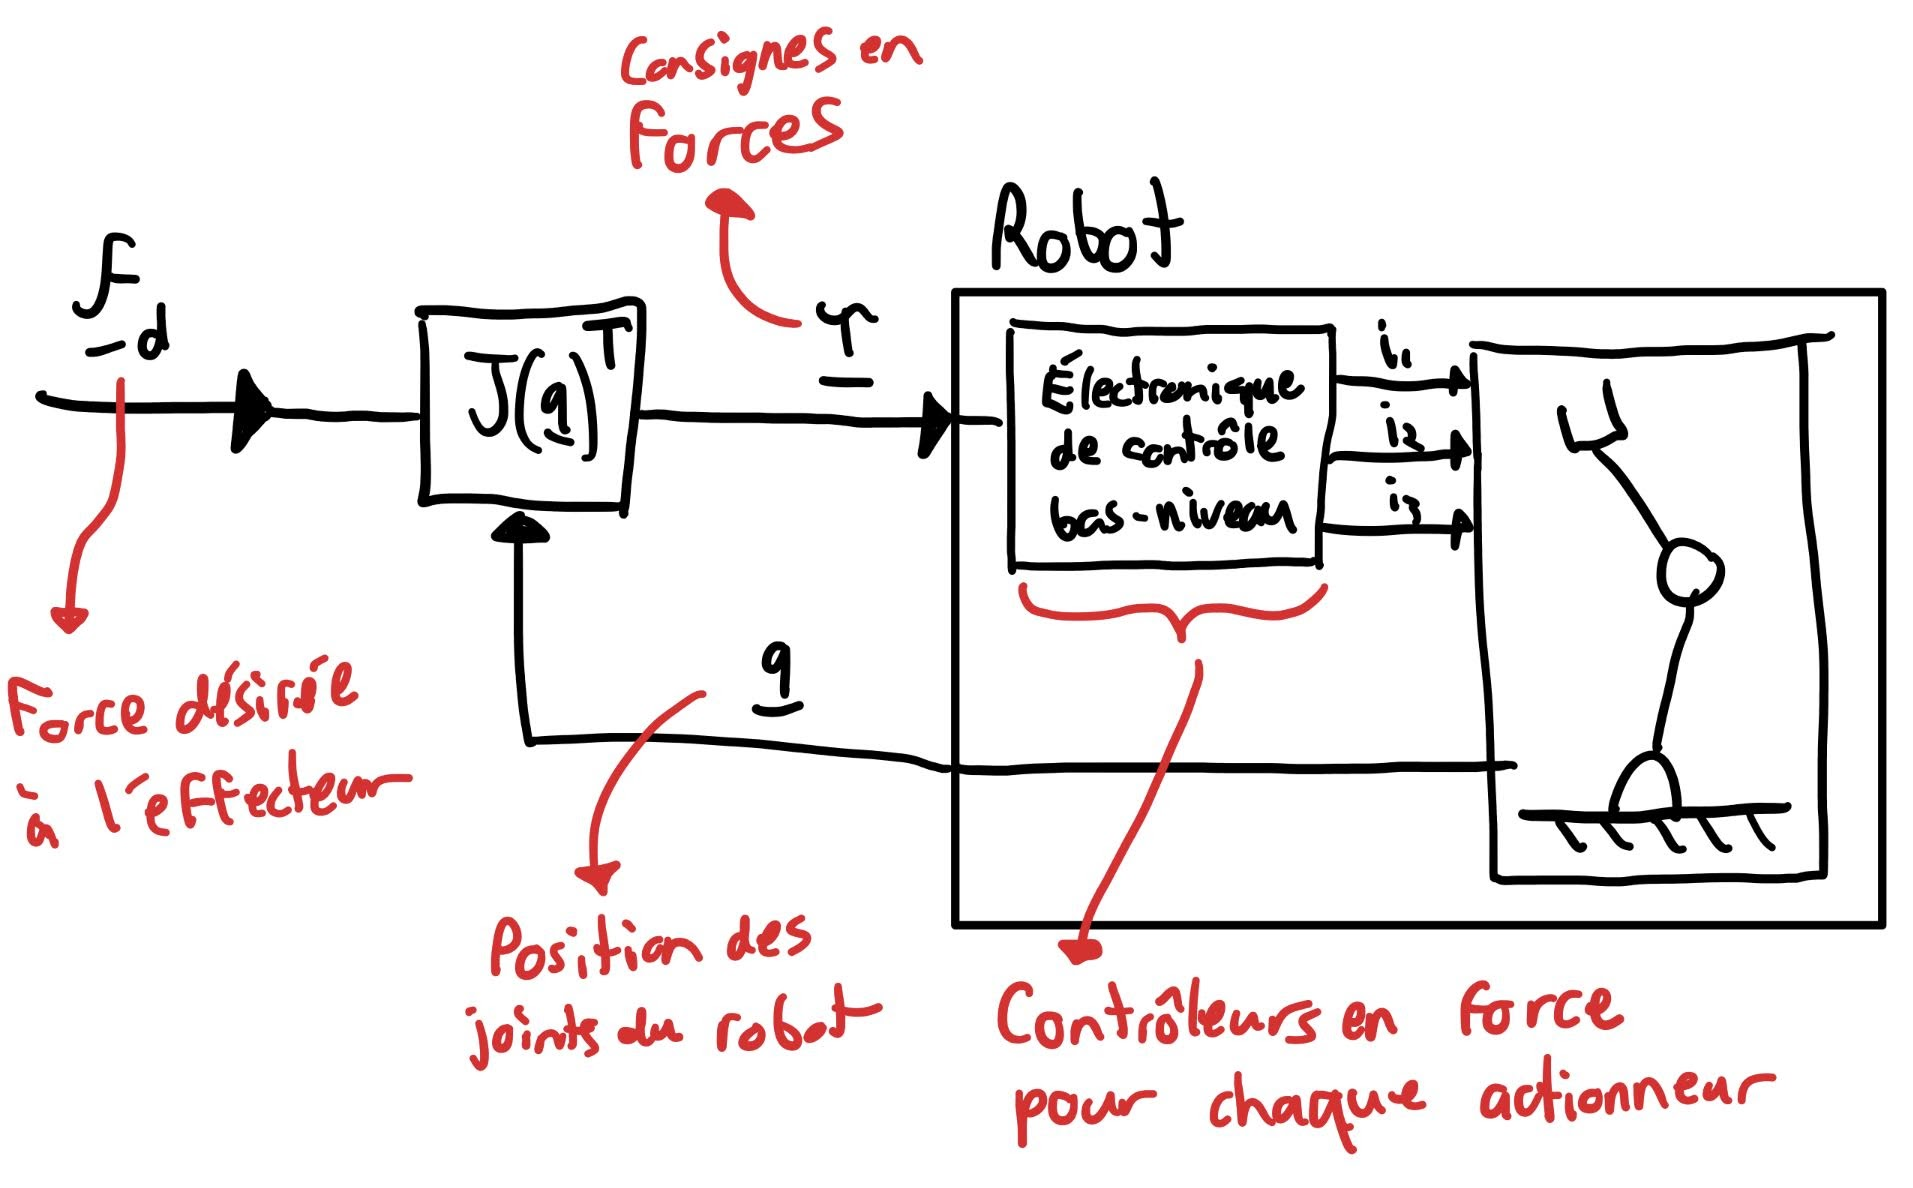
\includegraphics[width=0.60\textwidth]{fig/forcecontroleffectorbloc.jpg}
	\caption{Commande en force de l'effecteur d'un robot : schéma bloc}
	\label{fig:forcecontroleffectorbloc}
\end{figure}
%%%%%%%%%%%%%%%%%%%%%%%%%%%%%%%%

Il est à noter que pour produire une force, le principe action-réaction nous rappel qu'il faut avoir une résistance. Donc si l'effecteur n'est pas en contact avec un objet le comportement de cette loi de commande de donnera pas nécessairement le résultat attendu, les forces des actionneurs vont alors ce balancer avec la résistance interne du robot: forces dissipatrices et inertielles. Le robot va donc accélérer s'il n'y a pas de contact ou de résistance. Comme le mentionne le titre du chapitre, cette loi de commande \textbf{quasi-statique} fonctionne bien lorsque le robot est bloqué ou bien bouge très lentement, sinon les forces dissipatives et inertielles interne au robot vont influencer la force de contact. 



%%%%%%%%%%%%%%%%%%%%%%%%%%%%%%%%%%%%%%%%%%%%%%%%%%%%%%
%\newpage
\section{Commande en impédance et en admittance}
\label{sec:impcontrol}
%%%%%%%%%%%%%%%%%%%%%%%%%%%%%%%%%%%%%%%%%%%%%%%%%%%%%%

Jusqu'à maintenant, à la section \ref{sec:positioncontrol} une technique a été discutée pour contrôler la position d'un robot et à la section \ref{sec:forcecontrol} une technique a été discuté pour contrôler la force transmise par un robot. La dernière grande catégorie de type de commande est de contrôler la relation entre la positon et la force du robot. L'idée est d'imposer une loi de comportement qui relie la force au déplacement du système. Cette approche est particulièrement utile pour les situations ou un robot va entrer en contact avec un objet ou un humain. Un des inconvénients d'un contrôle en position pur est que si le robot rencontre un obstacle qui bloque son chemin, le robot va soudainement appliquer une très grande force pour tenter de continuer, ce qui peut risquer de briser soit l'objet rencontré ou le robot lui-même. À l'opposé, le problème avec une approche de contrôle en force pur est que si le robot n'a pas d'obstacle pour créer une résistance et établir la force désirée, le robot va plutôt accélérer jusqu'à se qu'il atteindre la limite de son espace de travail. La commande en impédance ou en admittance est une approche hybride qui vise plutôt à imposer une relation entre la force et le déplacement. Par exemple, on pourrait désirer que le robot se déplace de façon proportionnelle à une force appliqué sur celui-ci, en imposant ce comportement le robot émulerait le comportement d'un ressort. 

\video{Commande et impédance et admittance}{https://youtu.be/h_3qngSmwPo}

\textbf{Deux approches permettent d'imposer une relation entre la force et le mouvement d'un système}: la commande en impédance et en admittance. D'un point de vu théorique les approches sont pratiquement équivalentes, comme illustré à la Figure \ref{fig:impedanceadmitancecontrolbloc}, la différence est la causalité. Un contrôleur en impédance mesure le déplacement et impose une force, et un contrôleur en admittance mesure la force pour imposer un déplacement. Dans un monde idéal ou les mesures et le contrôle de la force/déplacement serait parfait, pour la même loi de comportement les deux approches donneraient un résultat identique. Toutefois, en pratique il y a de très grandes différences d'implémentation et de performance entre ces approches. 
%%%%%%%%%%%%%%%%%%%%%%%%%%%%%%%%%%%%%%%%%%%%%%%%%%%%%%%%%%%%%%%
\begin{figure}[H]
				%\vspace{-10pt}
        \centering
				\subfloat[Commande en \textbf{impédance}]{
				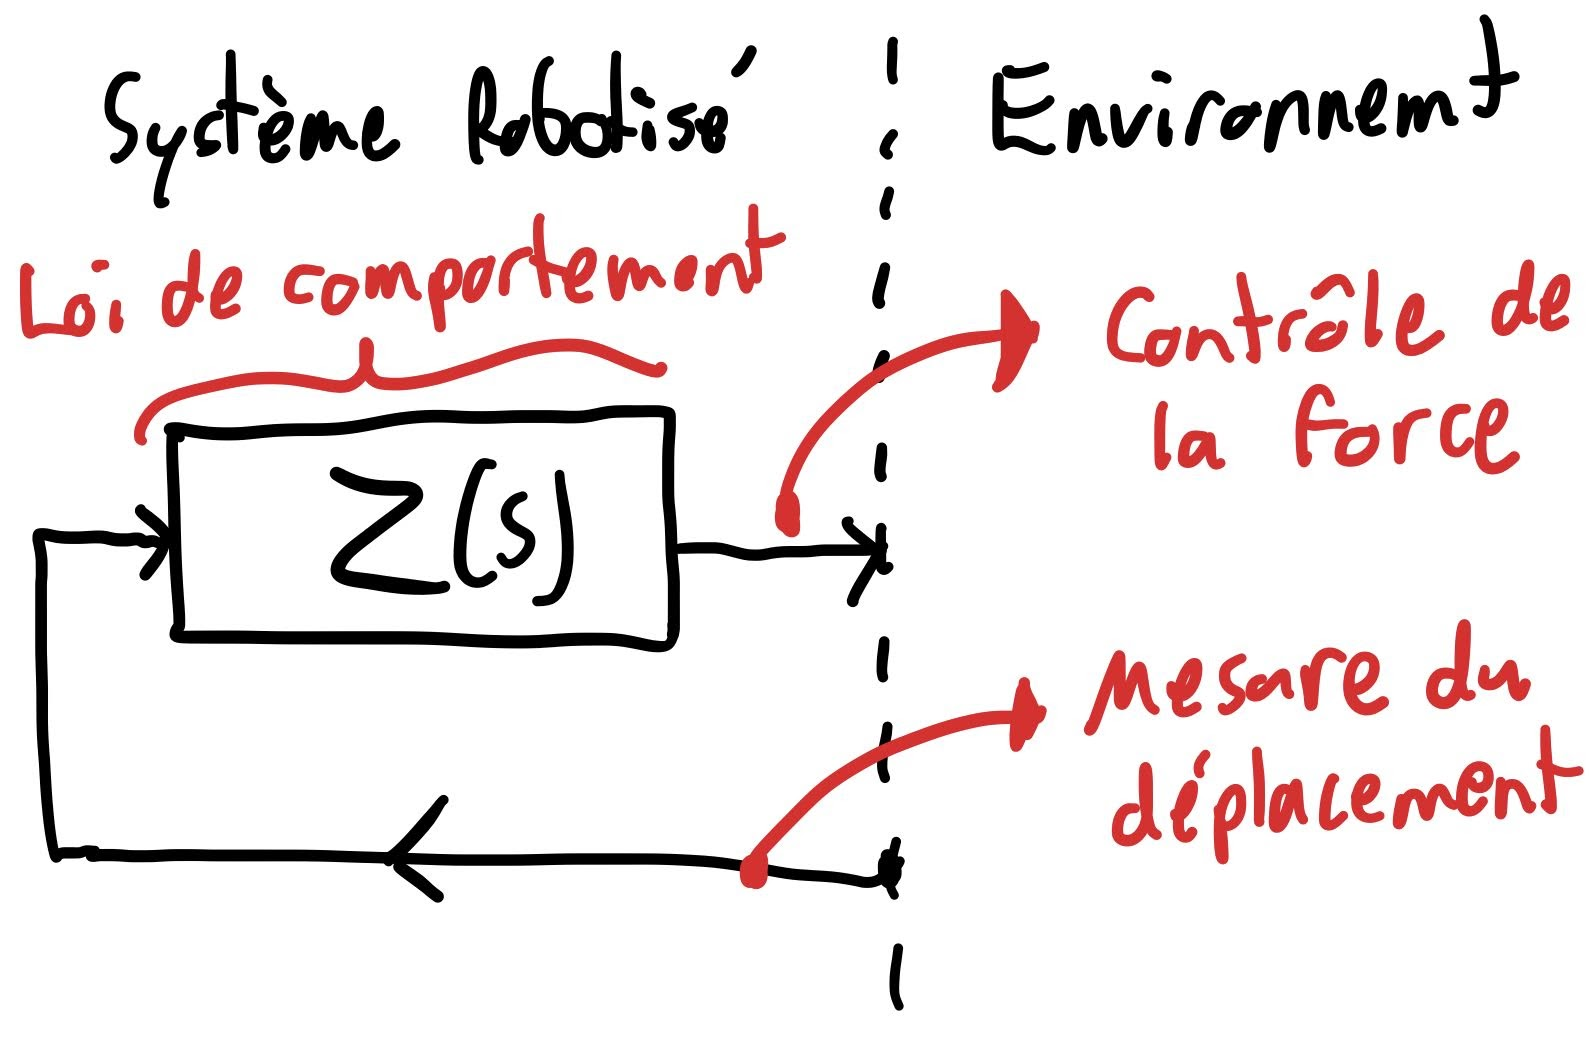
\includegraphics[width=0.40\textwidth]{fig/impedancecontrolbloc.jpg}
				\label{fig:impedancecontrolbloc}}
				%%%%
				\hspace{30pt}
				%%%%
				\subfloat[Commande en \textbf{admittance}]{
				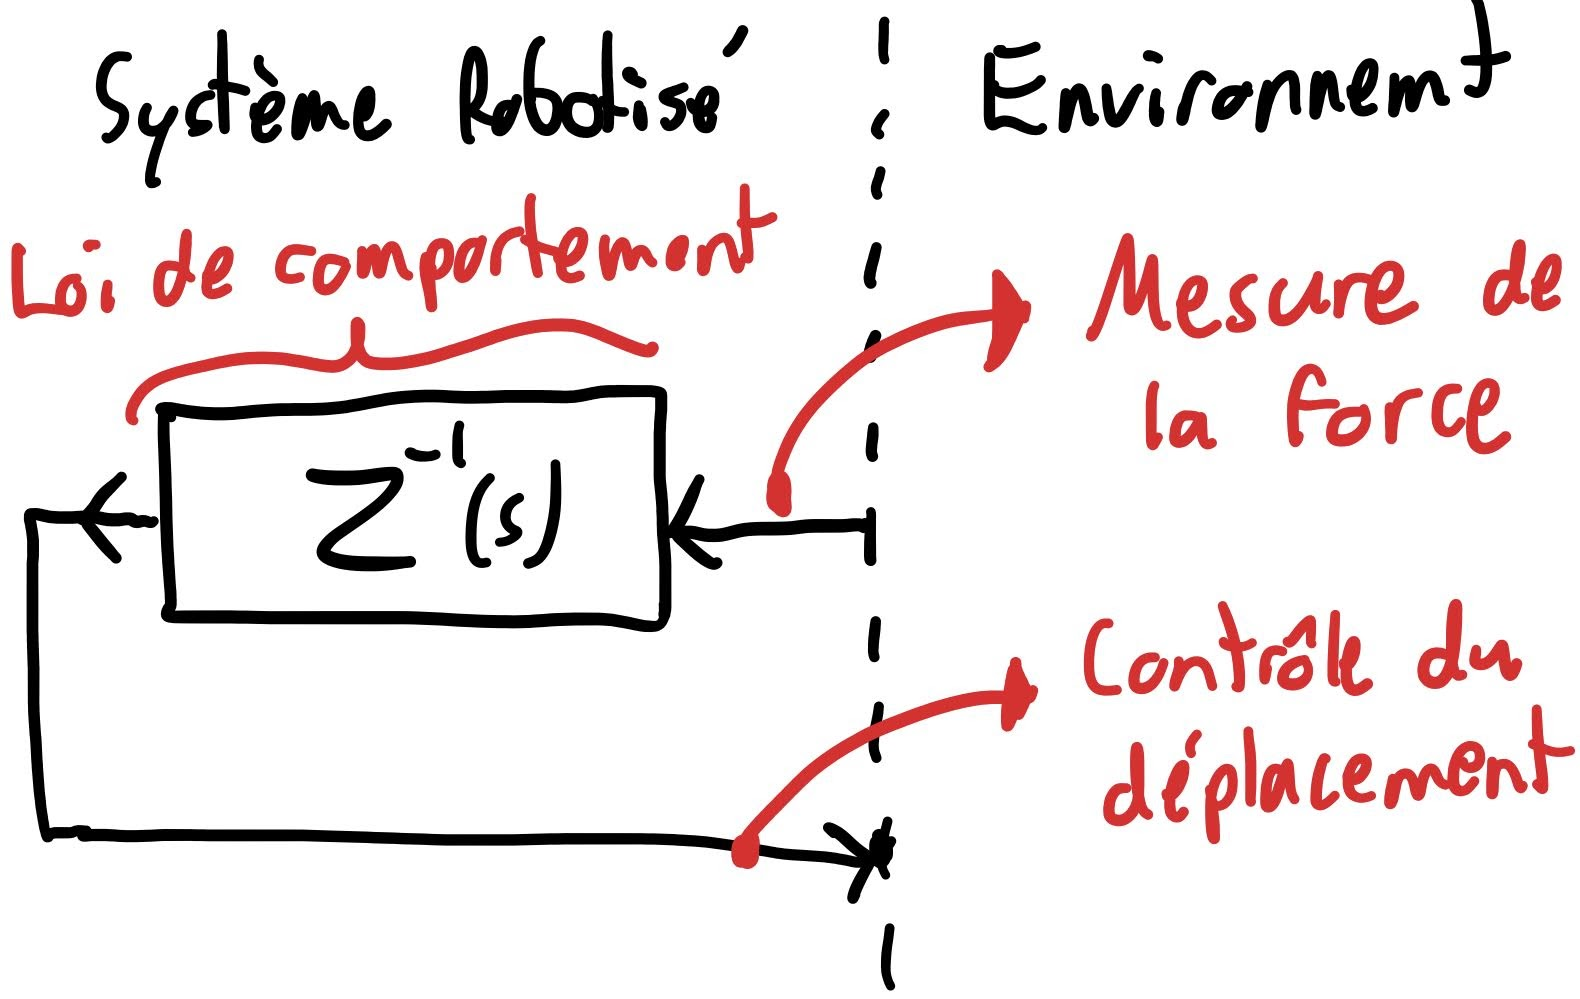
\includegraphics[width=0.40\textwidth]{fig/admitancecontrolbloc.jpg}
				\label{fig:admitancecontrolbloc}}
        \caption{Deux façon d'imposer une loi de comportement qui relie la force au déplacement.}
				\label{fig:impedanceadmitancecontrolbloc}
\end{figure}
%%%%%%%%%%%%%%%%%%%%%%%%%%%%%%%%%%%%%%%%%%%%%%%%%%%%%%%%%%%%%%%%%

Les lois de comportements mécaniques sont souvent décrit avec des fonctions de transfert dans le domaine de Laplace pour une notation compacte. La fonction $Z(s)$ est utilisée pour décrire l'impédance: le signal de force $f(s)$ divisé par le signal de déplacement $x(s)$ dans le domaine de Laplace. L'admittance $Y(s)$ est l'inverse de la fonction d'impédance. 
%%%%%%%%%%%%%%%%%%
\begin{align}
\text{Impédance:} \quad Z(s) = \frac{f(s)}{x(s)} \quad\quad \text{Admittance:} \quad Y(s) =  \frac{1}{Z(s)} = \frac{x(s)}{f(s)}
\end{align}
%%%%%%%%%%%%%%%%%

\note{Note:}{Dans certains ouvrage le concept d'impédance est définie comme la force divisée par la vitesse (contrairement à la position). La définition relative au déplacement sera toutefois utilisée ici car elle s'intègre plus naturellement au contexte de commande des robots.}

Un système mécanique avec une inertie $m$, un amortissement linéaire $b$ et une rigidité $k$ a une impédance complexe égale à:
%%%%%%%%%%%%%%%%%%
\begin{align}
Z(s) = m s^2 + b s + k 
\end{align}
%%%%%%%%%%%%%%%%%
L'opération de multiplié le signal de déplacement par l'impédance $Z(s)$ est équivalent dans le domaine temporel à :
%%%%%%%%%%%%%%%%%%
\begin{align}
f(s) = Z(s) x(s) = \left( m s^2 + b s + k \right) x(s) \quad \Longleftrightarrow \quad 
f(t) = m \frac{d^2}{dt^2} x(t) + b \frac{d}{dt} x(t) + k x(t) 
\end{align}
%%%%%%%%%%%%%%%%%


\paragraph{Exemple} Une loi de comportement qui est souvent désirable d'implémenter est la loi de \textit{Hooke}, i.e. un ressort. Comme illustré à la Figure \ref{fig:impedanceadmitancespring}, l'approche en impédance se résume à mesurer un signal de position $x$ et le multiplier par une constante de rigidité $k$ pour obtenir la force à appliquer. L'approche en admittance se résume à mesurer un signal de force $f$ et le diviser par la constante de rigidité $k$ pour obtenir le déplacement $x$ à imposer. On utilise parfois la notion de compliance $C=1/k$ qui est l'inverse de la rigidité. 
%%%%%%%%%%%%%%%%%%%%%%%%%%%%%%%%%%%%%%%%%%%%%%%%%%%%%%%%%%%%%%%
\begin{figure}[H]
				\vspace{-10pt}
        \centering
				\subfloat[Commande en \textbf{impédance}]{
				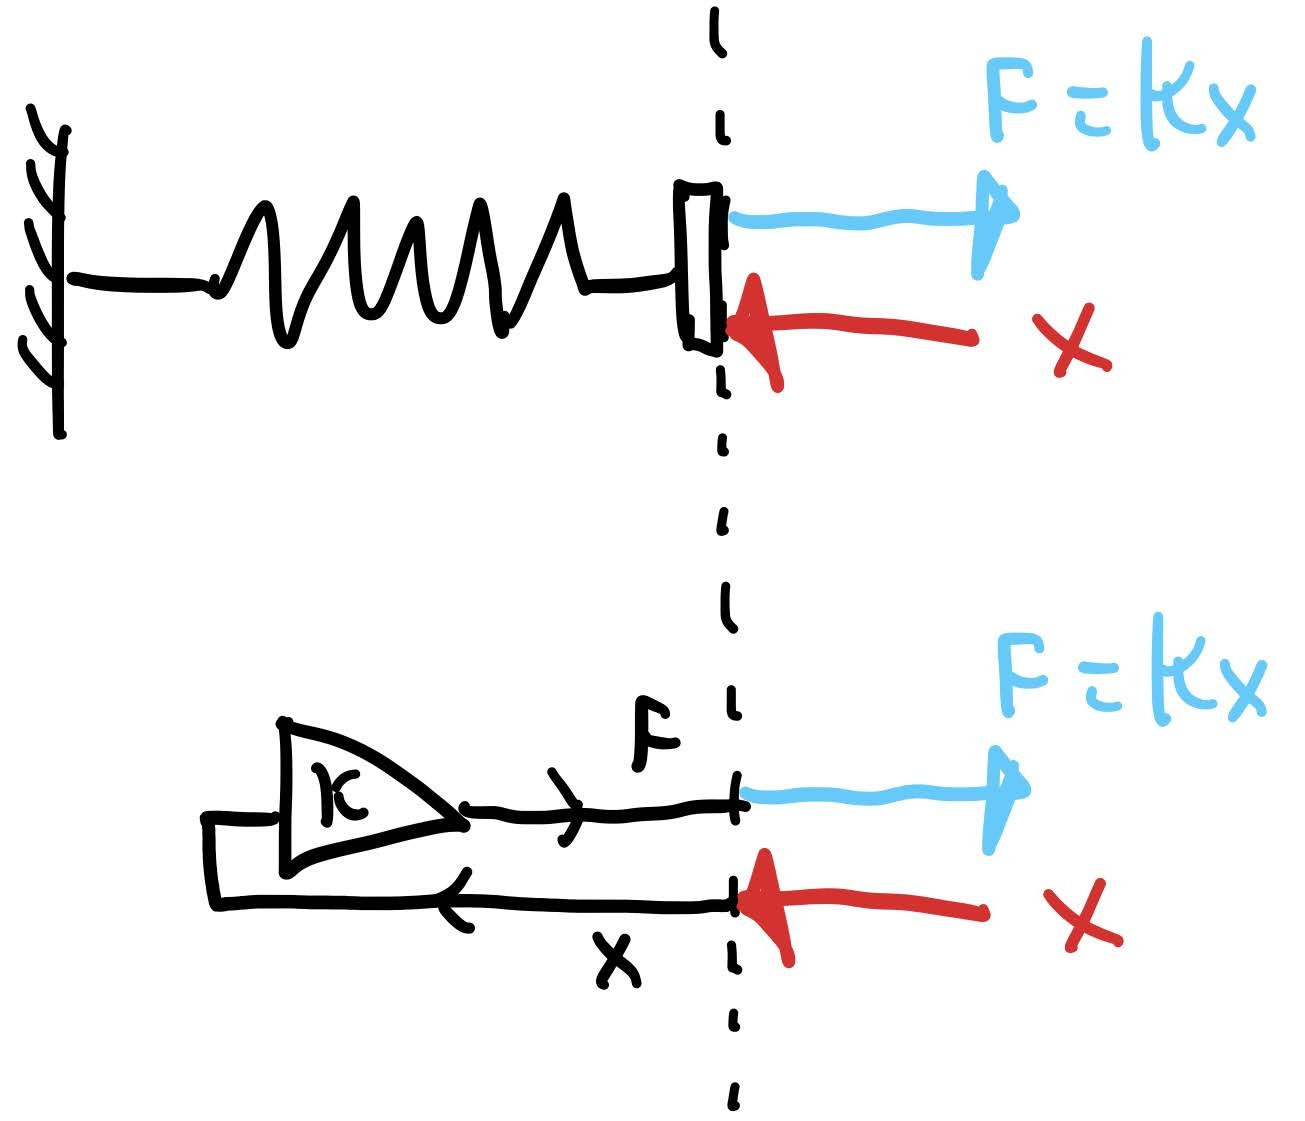
\includegraphics[width=0.35\textwidth]{fig/impedancecontrolspring.jpg}
				\label{fig:impedancecontrolspring}}
				%%%%
				\hspace{5pt}
				%%%%
				\subfloat[Commande en \textbf{admittance}]{
				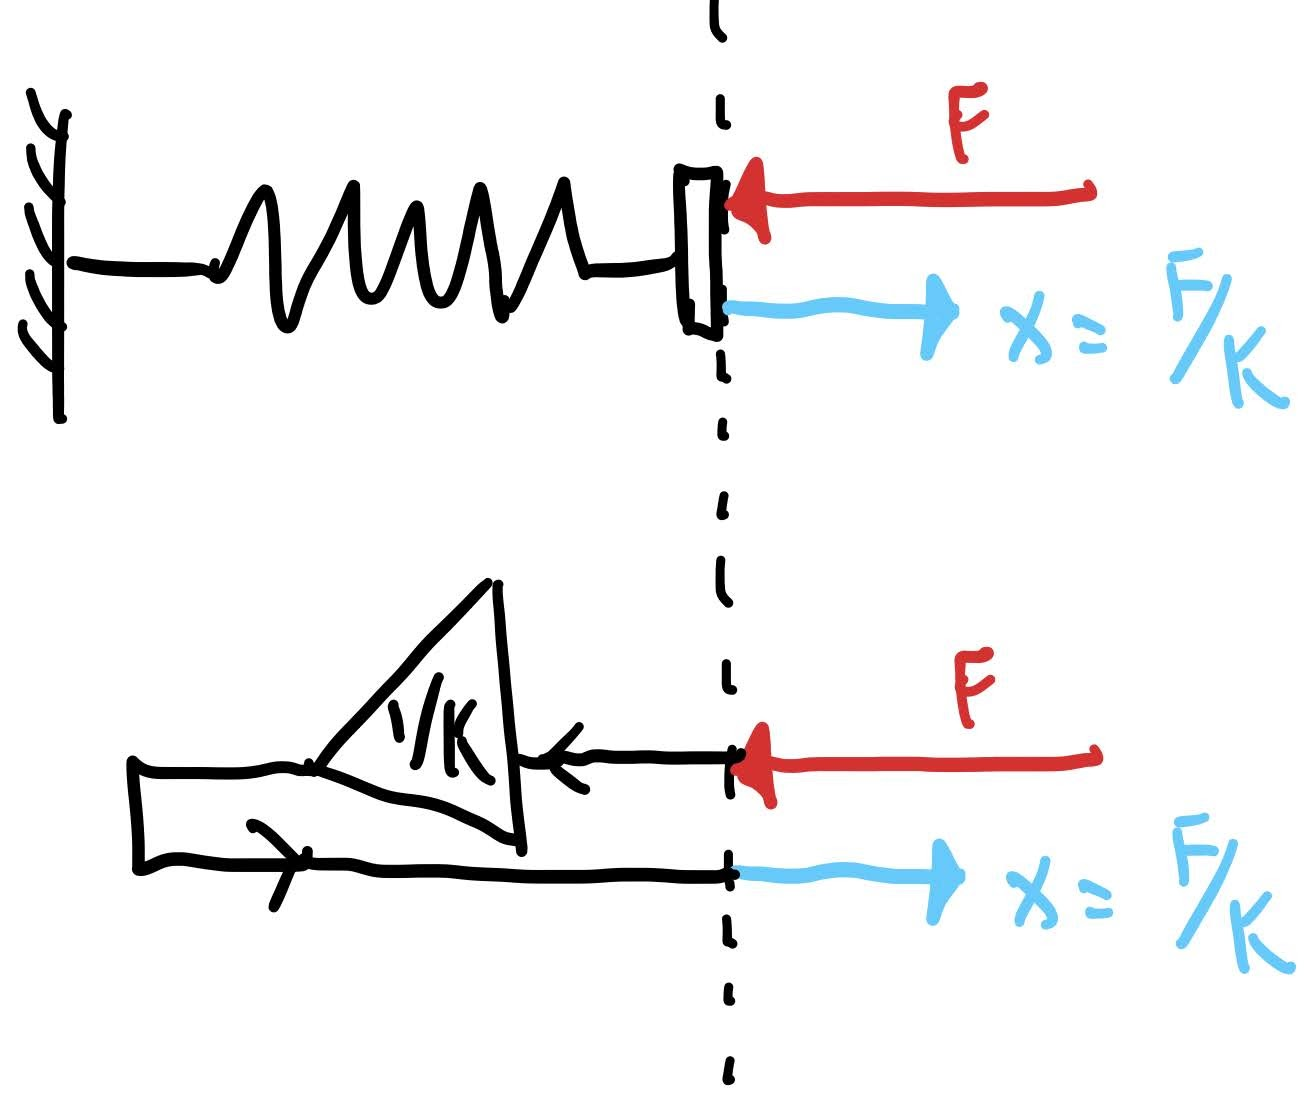
\includegraphics[width=0.35\textwidth]{fig/admitancecontrolspring.jpg}
				\label{fig:admitancecontrolspring}}
        \caption{Imposition d'une loi de comportement $f=kx$ (ressort)}
				\label{fig:impedanceadmitancespring}
\end{figure}
%%%%%%%%%%%%%%%%%%%%%%%%%%%%%%%%%%%%%%%%%%%%%%%%%%%%%%%%%%%%%%%%%

En pratique, se qui va guider le choix d'une approche ou d'une autre est principalement le type d'actionneur utilisé dans le système robotisé. L'approche par impédance est plus naturelle pour un système avec des actionneurs qui sont des sources de forces (moteur électrique sans réducteur, cylindre pneumatique, etc.), tandis que l'approche par admittance est plus naturelle pour les systèmes avec des actionneurs qui sont des sources de déplacement, i.e. plus facilement contrôlable en position ou vitesse comme la plupart des moteurs électriques jumelés à des grandes réductions utilisés dans les robots industriels. La Figure \ref{fig:impedanceadmitancesex} illustre deux implémentations possibles pour émuler la loi de \textit{Hooke}.
%
Généralement, l'approche en impédance jumelée à des actionneurs à faible résistance hautement réversible (source de force pure) est idéale pour bien émuler des loi de comportement caractérisés par des petites impédances. La performance est toutefois limitée pour émuler des rigidités très élevée. Cette approche est généralement utilisée par les systèmes haptiques et certains systèmes robotiques collaboratif. À l'inverse, l'approche en admittance avec des actionneurs irréversibles (source de position), est idéale pour émuler de très grandes impédances. La performance est toutefois limitée pour émuler un comportement très compliant (peu de résistance) car l'accélération et la vitesse des actionneurs sont limités en pratique. Cette approche est généralement utilisée par les robots collaboratifs industriels. 
%%%%%%%%%%%%%%%%%%%%%%%%%%%%%%%%%%%%%%%%%%%%%%%%%%%%%%%%%%%%%%%
\begin{figure}[H]
				\vspace{-10pt}
        \centering
				\subfloat[Commande en \textbf{impédance}]{
				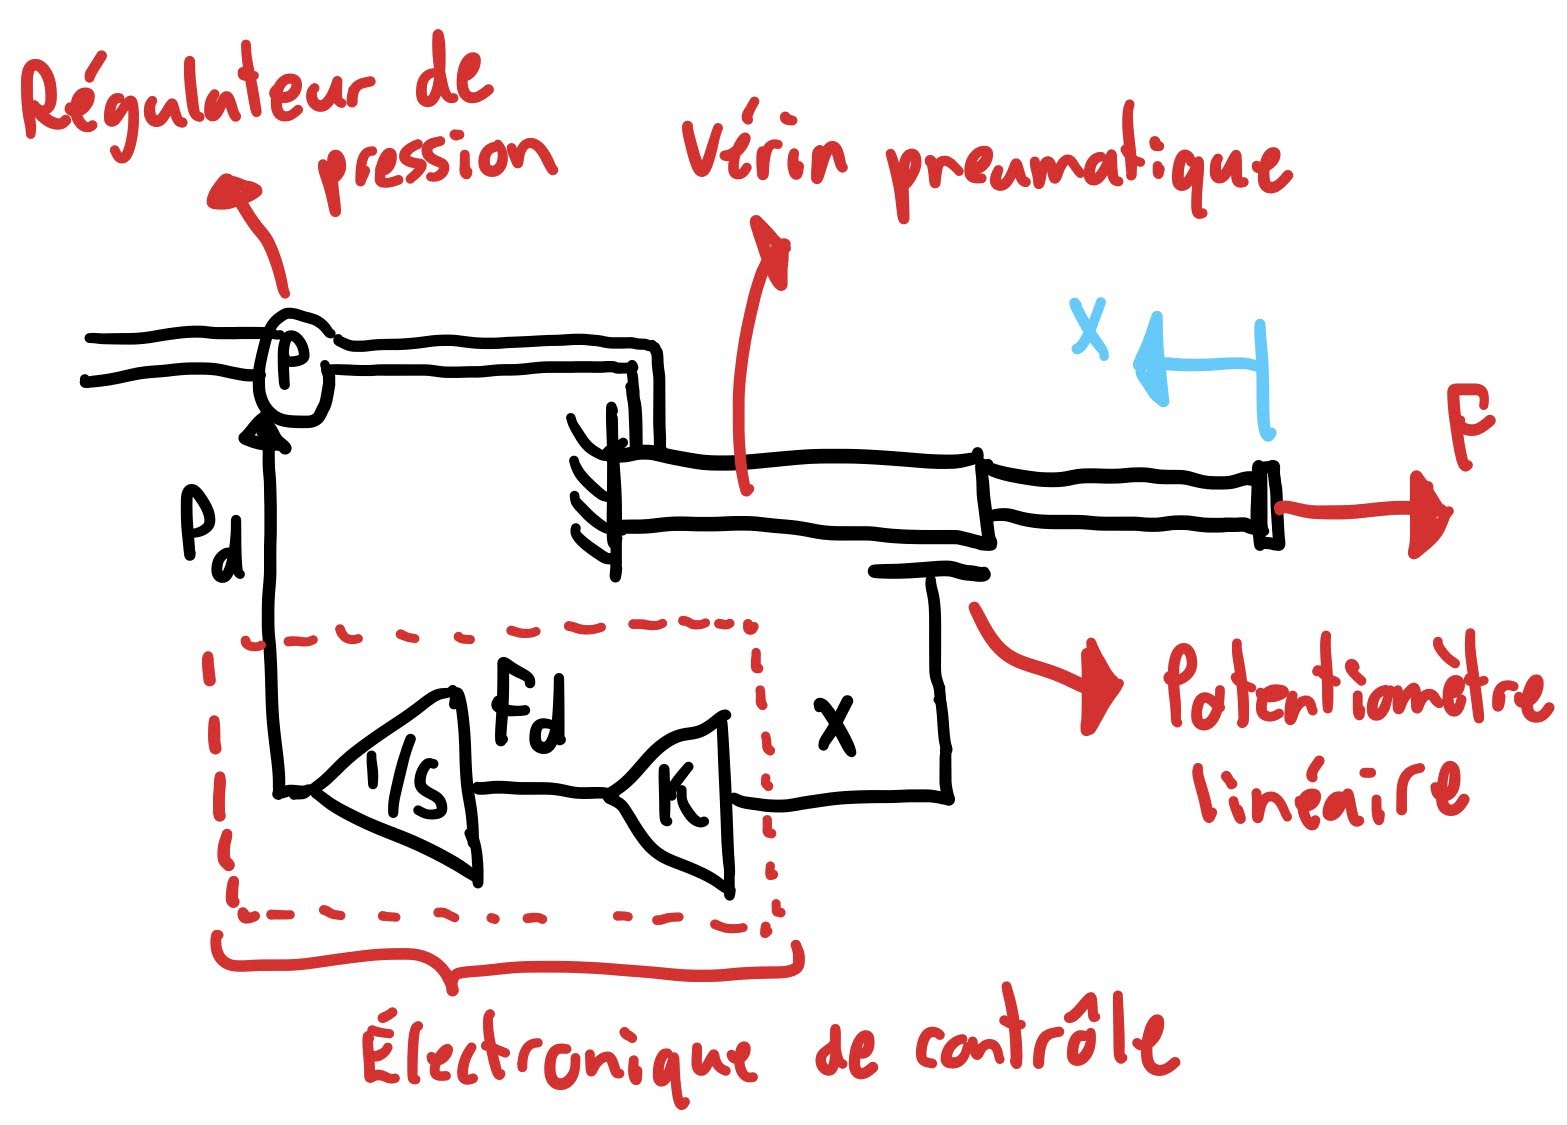
\includegraphics[width=0.45\textwidth]{fig/impedancecontrolpiston.jpg}
				\label{fig:impedancecontrolpiston}}
				%%%%
				\hspace{5pt}
				%%%%
				\subfloat[Commande en \textbf{admittance}]{
				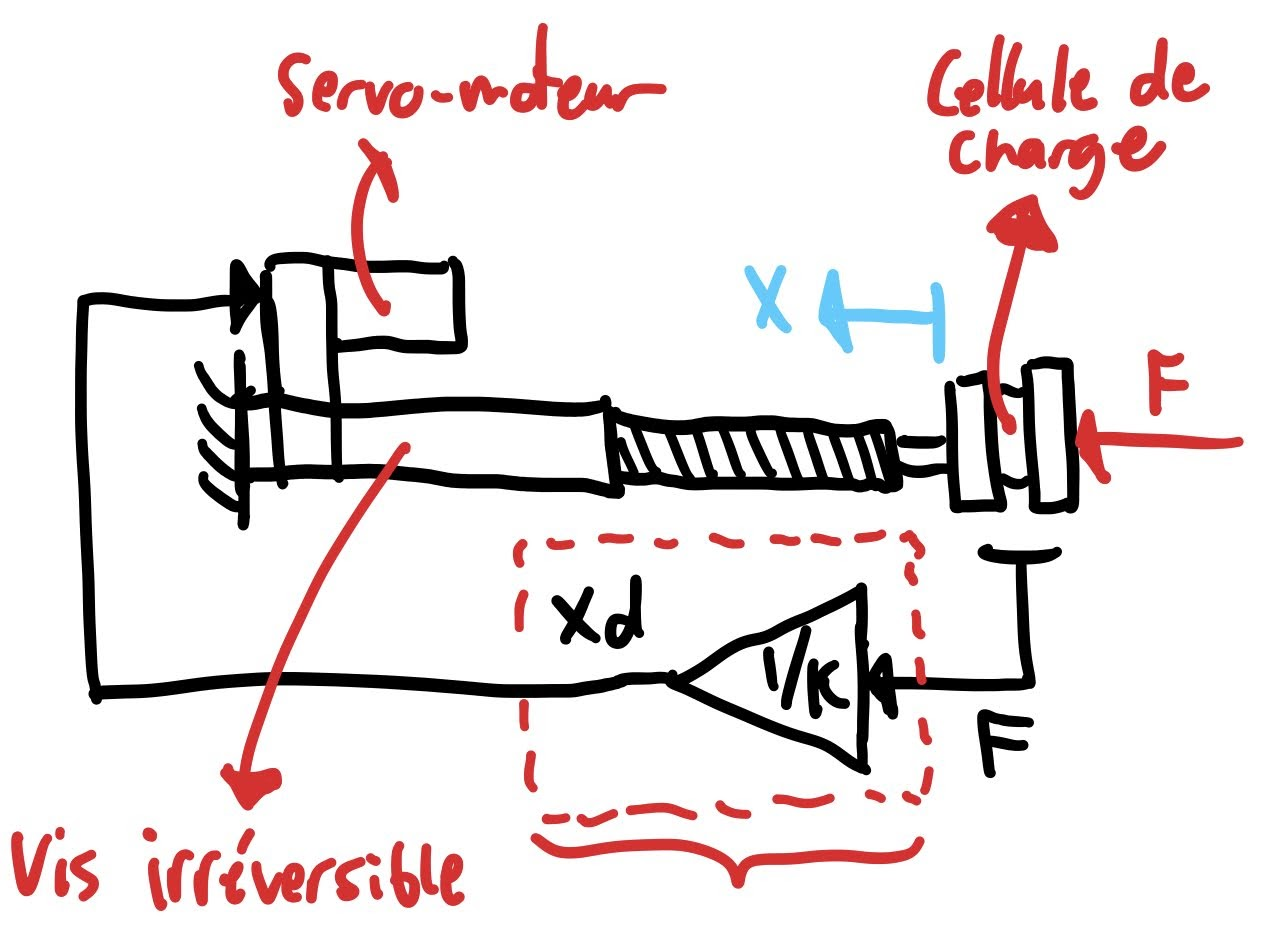
\includegraphics[width=0.45\textwidth]{fig/admitancecontrolservo.jpg}
				\label{fig:admitancecontrolservo}}
        \caption{Deux exemples d'implémentation de commande pour une loi de comportement $f=kx$ (ressort). L'approche en impédance est adaptée à aux actionneurs qui sont des sources de force avec peu de résistance interne. L'approche en admittance est adaptée aux actionneurs qui sont irréversibles et donc des sources de déplacements peu influencées par la résistance externe.}
				\label{fig:impedanceadmitancesex}
\end{figure}
%%%%%%%%%%%%%%%%%%%%%%%%%%%%%%%%%%%%%%%%%%%%%%%%%%%%%%%%%%%%%%%%%

Les sections suivantes présentent des approches de commande haut-niveau, i.e. la coordination spatiale de plusieurs joints pour obtenir des lois de comportement, soit exprimées dans l'espace des joints ou de la tâche comme illustré à la Figure \ref{fig:stiffnesscontrol}. Dans ces sections il est considéré que les actionneurs sont soit des sources parfaites de force ou des sources parfaites de déplacement. La performance dynamique des boucles en forces/impédance/admittance implique une analyse de la dynamique bas-niveau des actionneurs qui est plutôt traité au chapitre \ref{sec:actuatorcontrol}. 

%%%%%%%%%%%%%%%%%%%%%%%%%%%%%%%%%%%%%%%%%%%%%%%%%%%%%%%%%%%%%%%
\begin{figure}[H]
				%\vspace{-10pt}
        \centering
				\subfloat[Dans l'espace des joints]{
				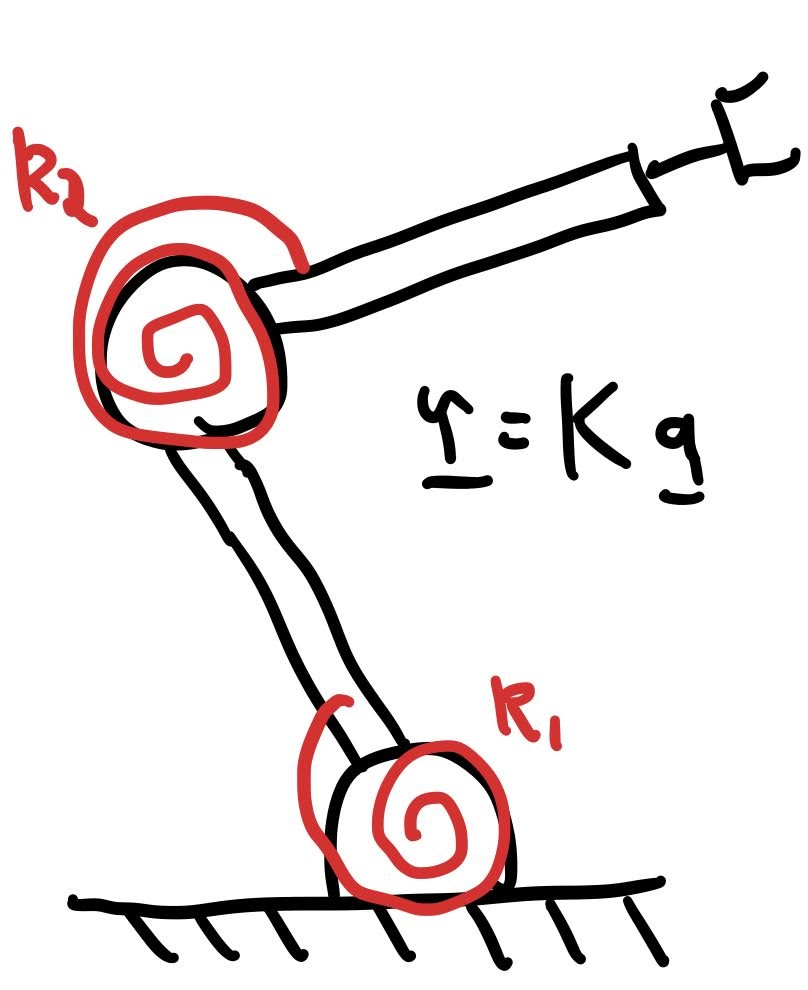
\includegraphics[width=0.30\textwidth]{fig/jointspacestiffness.jpg}
				\label{fig:jointspacestiffness}}
				%%%%
				\hspace{5pt}
				%%%%
				\subfloat[Dans l'espace de la tâche]{
				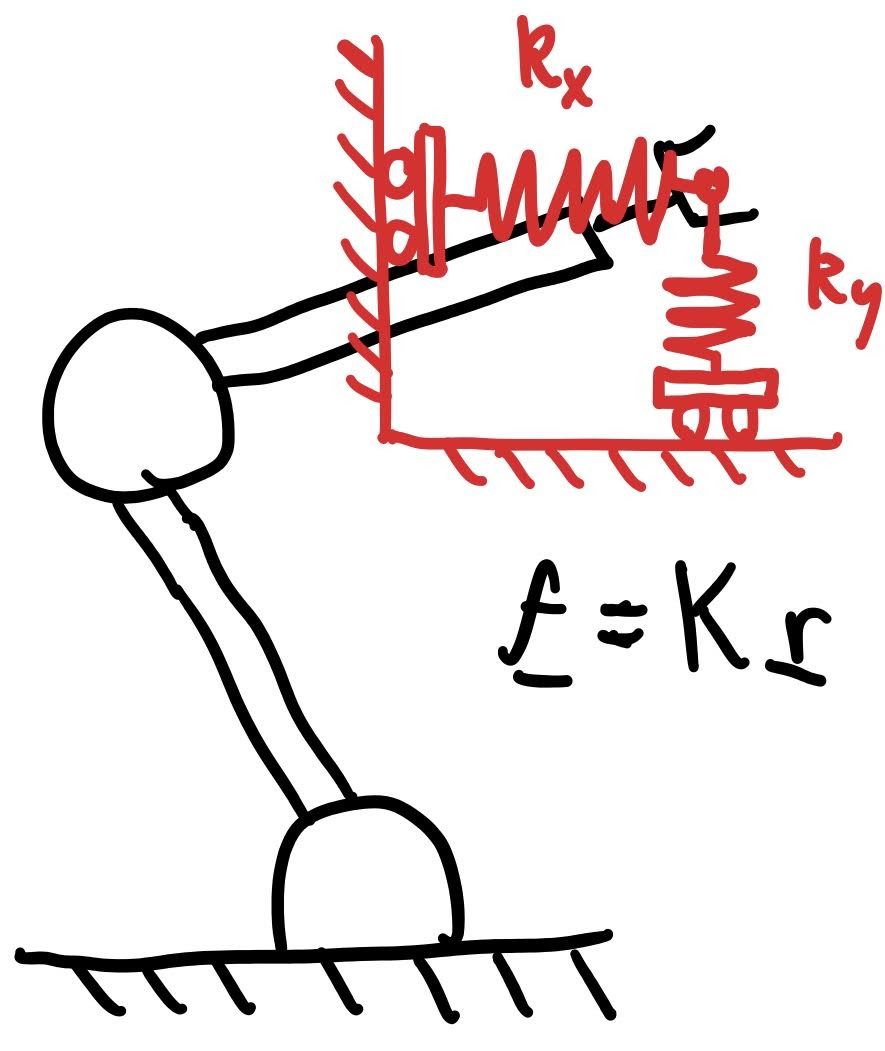
\includegraphics[width=0.30\textwidth]{fig/taskspacestiffness.jpg}
				\label{fig:taskspacestiffness}}
        \caption{Commande de la rigidité/compliance d'un robot}
			\label{fig:stiffnesscontrol}
\end{figure}
%%%%%%%%%%%%%%%%%%%%%%%%%%%%%%%%%%%%%%%%%%%%%%%%%%%%%%%%%%%%%%%%%


%%%%%%%%%%%%%%%%%%%%%%%%%%%%%%%%%%%%%%%%%%%%%%%%%%%%%%%%%%%%%%%%%
\subsection{Commande en impédance aux joints}
\label{sec:jointimpcontrol}

Pour des robots avec des actionneurs contrôlés en force ou couple, la commande en impédance aux joints se résume à relié le déplacement mesuré aux joints aux efforts à chaque joint. Dans le cas le plus simple, comme illustré à la Figure \ref{fig:jointspacestiffness}, on peut commander des couples moteurs proportionnel aux déplacement angulaire des joints, ce qui est équivalent à émuler des ressorts angulaires sur chaque joint. De façon général on pourrait émuler des ressorts-amortisseurs sur chaque joint avec la loi de commande:
%%%%%%%%%%%%%%%%%%
\begin{align}
\col{\tau} = K \col{q}_e + B \col{\dot{q}}_e
\label{eq:jointspaceimpe}
\end{align}
%%%%%%%%%%%%%%%%%
ou $\col{q}_e = \col{q}_d - \col{q}$ est une erreur par rapport à la configuration de référence ou les ressorts sont "au repos". Les matrices $K$ et $B$ sont respectivement une matrice de coefficients de rigidité et une matrice de coefficients d'amortissement. Les matrice sont diagonales pour un comportement de chaque joint indépendant. Dans ce cas diagonal, la loi de commande est équivalente à plusieurs boucle d'asservissement indépendantes de type Proportionnel-Dérivé sur la position des joints. La loi de commande est illustrée sous forme de schéma bloc à la Figure \ref{fig:impedancecontroljoint}.
%%%%%%%%%%%%%%%%%%%%%%%%%%%%%%%%
\begin{figure}[h]
	\centering
		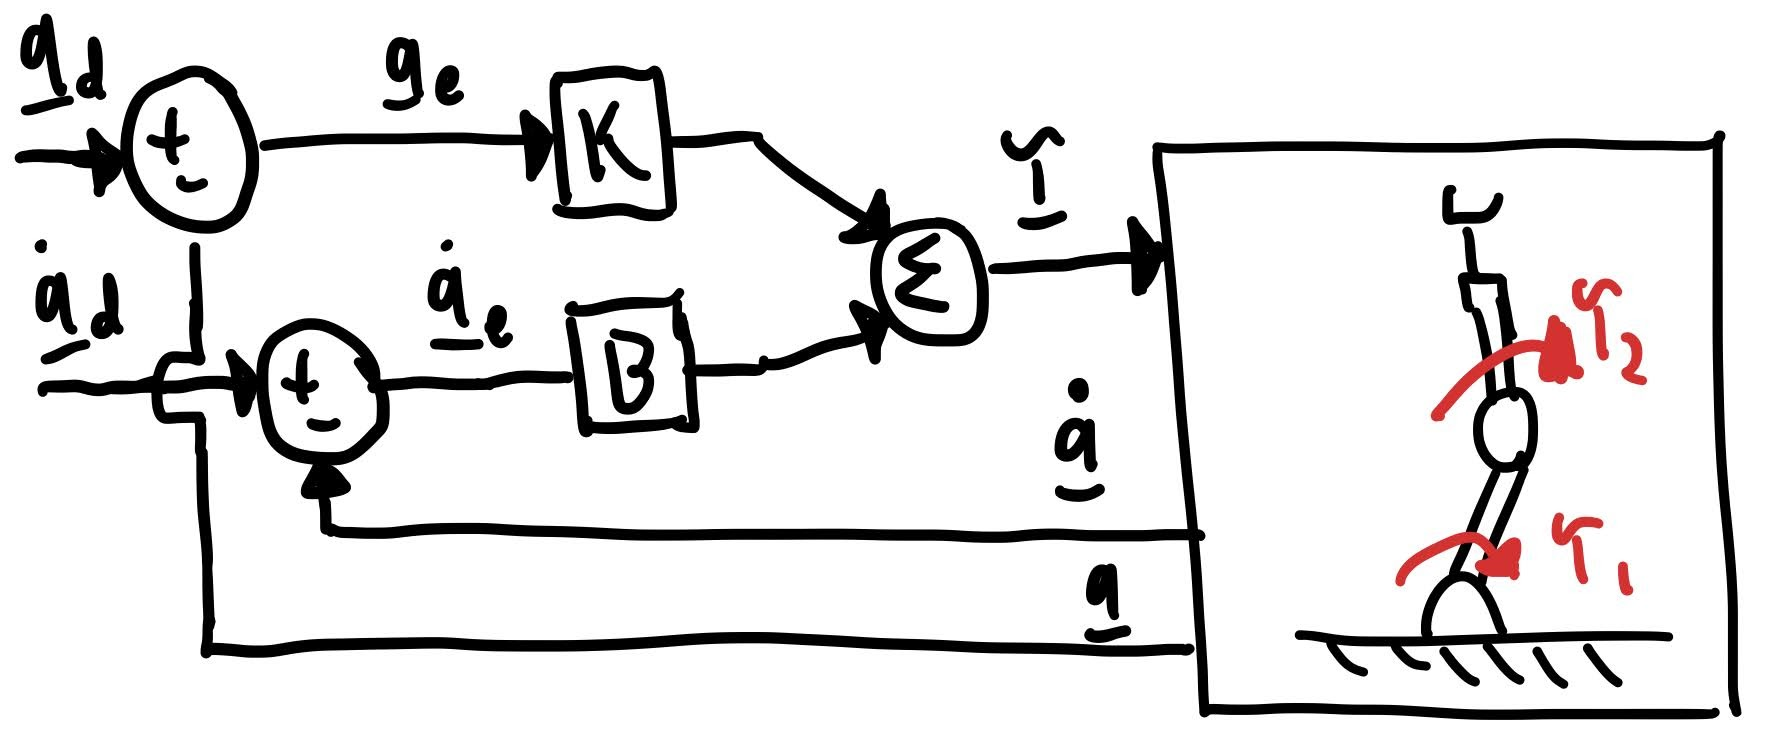
\includegraphics[width=0.6\textwidth]{fig/impedancecontroljoint.jpg}
	\caption{Commande de l'impédance au joints d'un robot: schéma bloc}
	\label{fig:impedancecontroljoint}
\end{figure}
%%%%%%%%%%%%%%%%%%%%%%%%%%%%%%%%
Comme ici on programme des lois de comportement, il est possible de programmer des impédances non-linéaires arbitraires. Par exemple, pour les systèmes haptiques un problème courant est d'émuler un obstacle rigide, ce qui est appeler mur virtuel dans la littérature. L'impédance cible dans ce cas est discontinue, aucune résistance pour une certaine plage de déplacement et une très grand rigidité lorsque la position atteint la position du mur virtuel.

\textbf{Compensation de friction: } Les systèmes robotiques vont normalement avoir de la dissipation naturelle présente dans les joints (roulements, engrenage, etc.). Si la friction naturelle est significative et plus grande que l'amortissement qu'on désire émuler, les coefficients de friction dans $B$ pourraient être négatif pour appliquer une force opposée à la friction naturelle. La matrice $B$ pourrait être définie par:
%%%%%%%%%%%%%%%%
\begin{align}
B = B_{d} - B_{sys}
\end{align}
%%%%%%%%%%%%%%%%%
ou $B_{d}$ contient les coefficients d'amortissement que l'on désire émuler et $B_{sys}$ contient les coefficients d'amortissement naturel du robot. Il est toutefois risqué en pratique de tenter de totalement compenser la friction dans les joints d'un robot, car si la compensation est légèrement plus forte que la friction naturelle le système se retrouve instable. De plus le comportement de la friction autour de zéro vitesse est généralement très non-linéaire et avec de l'hystérésis, donc dur à modéliser avec précision. 

\note{Note sur l'émulation de l'inertie: }{ On pourrait être tenté de rajouter un terme de type $M \col{\ddot{q}}_e$ à l'équation \eqref{eq:jointspaceimpe} pour rajouter l'option d'émuler un effet inertiel sur chaque joint. Toutefois il y a un problème de causalité à une telle opération. L'accélération n'est pas un état du système mais résulte de l'application de forces sur le système incluant $\col{\tau}$. Donc les couples dépendraient de l'accélération mesurée, qui dépend des couples appliquées par les actionneurs, qui dépendraient de l'accélération mesurée, qui dépend ... etc. On se retrouve avec une boucle algébrique analogue au paradoxe de la poule et de l'oeuf (lequel vient en premier?). En pratique, l'accélération mesurée serait celle d'un instant passé dû au délai de calcul dans le contrôleur et aux filtres dans les capteurs, et la rétroaction de la mesure de l'accélération risque de déstabiliser le système.}

%%%%%%%%%%%%%%%%%%%%%%%%%%%%%%%%%%%%%%%%%%%%%%%%%%%%%%%%%%%%%%%%%
\subsection{Commande en impédance de l'effecteur}
\label{sec:effimpcontrol}

Pour la commande en impédance de l'effecteur d'un robot, c'est la relation force-déplacement à l'effecteur qu'on impose au robot:
%%%%%%%%%%%%%%%%%%
\begin{align}
\col{f}_e  =  K \col{r}_e + B \col{\dot{r}}_e 
\end{align}
%%%%%%%%%%%%%%%%%
ou $\col{r}_e = \col{r}_d - \col{r} $ est le vecteur position qui de la position désirée de l'effecteur du robot par rapport à la position actuelle. On peut interpréter l'effet de la loi de commande comme un ressort-amortisseur virtuel qui relit l'effecteur du robot à sa position cible comme illustré à la Figure \ref{fig:impedanceeffectorgeo}.
%%%%%%%%%%%%%%%%%%%%%%%%%%%%%%%%
\begin{figure}[h]
	\centering
		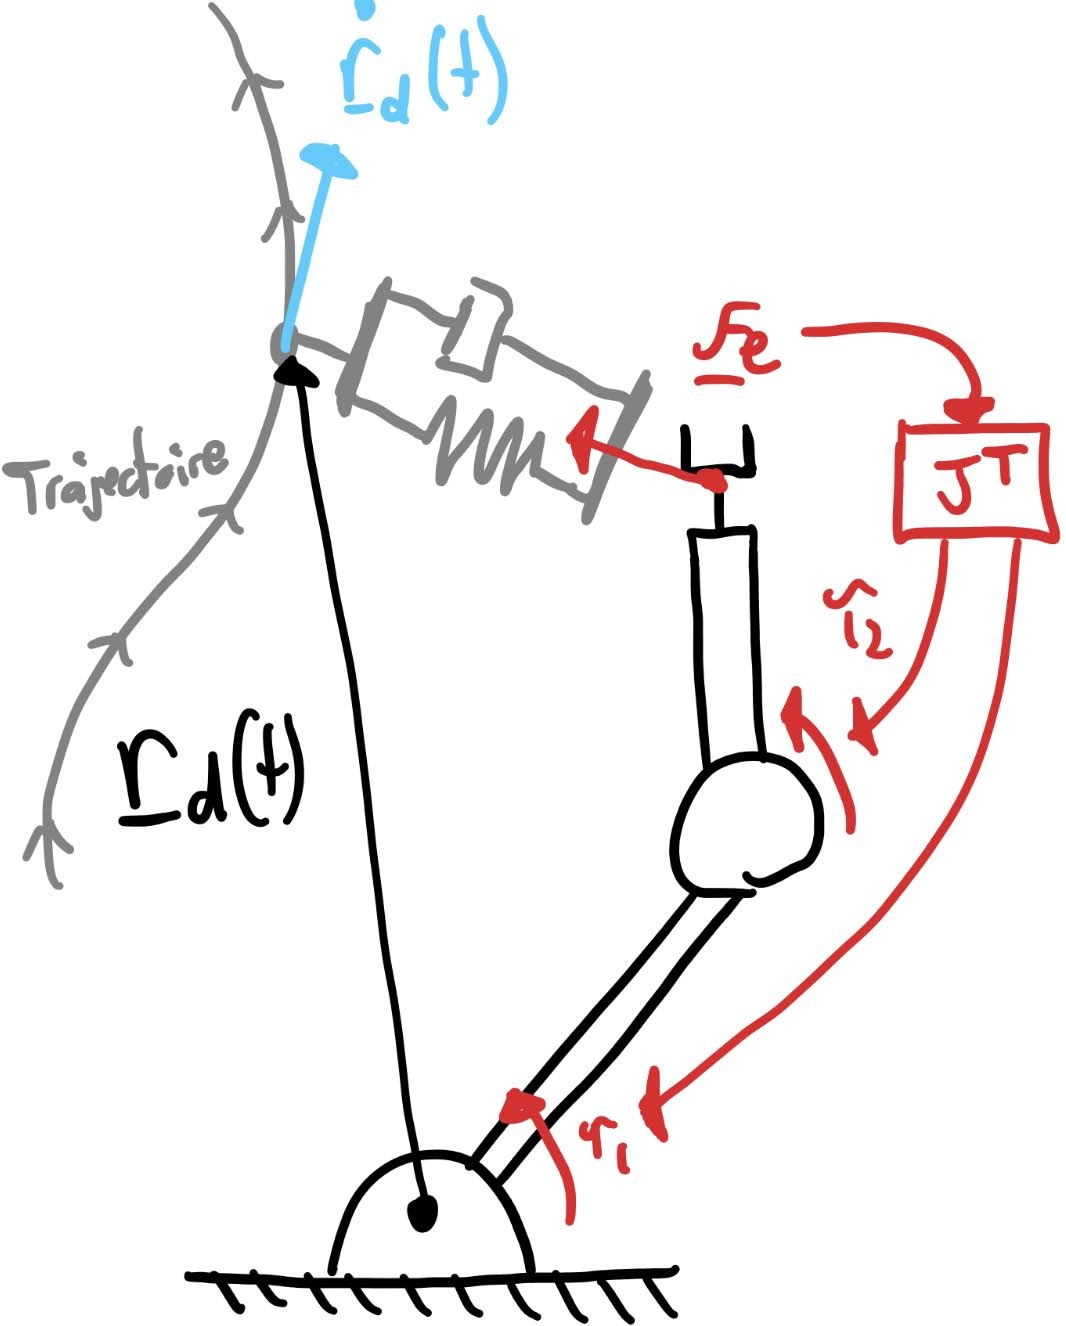
\includegraphics[width=0.4\textwidth]{fig/impedancecontroleffectorgeo.jpg}
	\caption{Commande de l'impédance de l'effecteur d'un robot : interprétation géométrique}
	\label{fig:impedanceeffectorgeo}
\end{figure}
%%%%%%%%%%%%%%%%%%%%%%%%%%%%%%%%
Le ressort-amortisseur virtuel produit une force virtuelle $\col{f}_e$ désirée à l'effecteur qui est traduite en commande de couple grâce à la relation statique d'un manipulateur:
%%%%%%%%%%%%%%%%%%
\begin{align}
\col{\tau} &= J(\col{q})^T \col{f}_e
\end{align}
%%%%%%%%%%%%%%%%%

\video{Commande en impédance d'un robot manipulateur}{https://youtu.be/Rl2kDwsYS9E}

La Figure \ref{fig:impedanceeffectorbloc} illustre cette loi de commande avec un schéma bloc. La première étape du contrôleur est de calculer la position et la vitesse de l'effecteur à partir des capteurs qui mesurent la position et la vitesse des joints. Il faut donc ici utiliser la cinématique directe et la cinématique-différentielle directe pour calculer la position et la vitesse de l'effecteur. Ensuite la position et la vitesse de l'effecteur sont comparées à la position et la vitesse désirée (qui peut varier dans le temps, i.e. une trajectoire). L'erreur en termes de position et vitesse est convertie en force cartésienne basé sur la loi de comportement désirée (l'impédance è l'effecteur). Finalement cette force cartésienne est convertie en couple aux joints grâce au Jacobien du robot manipulateur. On peut aussi ajouter une compensation de gravité, voir la section \ref{sec:impcontrolconvergence}. L'équation de la loi de commande est égale à:
%%%%%%%%%%%%%%%%%%
\begin{align}
\col{\tau} &= J(\col{q})^T \col{f}_e \\
\col{\tau} &= J(\col{q})^T   \left[ K \col{r}_e + B \col{\dot{r}}_e \right] \\
\col{\tau} &= J(\col{q})^T  \left[ K  \left( \col{r}_d- \col{r} \right) + B  \left( \col{\dot{r}}_d - \col{\dot{r}} \right)  \right] \\
\col{\tau} &= J(\col{q})^T  \left[ K  \left( \col{r}_d- f(\col{q}) \right) + B  \left( \col{\dot{r}}_d - J(\col{q}) \col{\dot{q}} \right)  \right] 
\end{align}
%%%%%%%%%%%%%%%%%
%%%%%%%%%%%%%%%%%%%%%%%%%%%%%%%%
\begin{figure}[th]
	\centering
		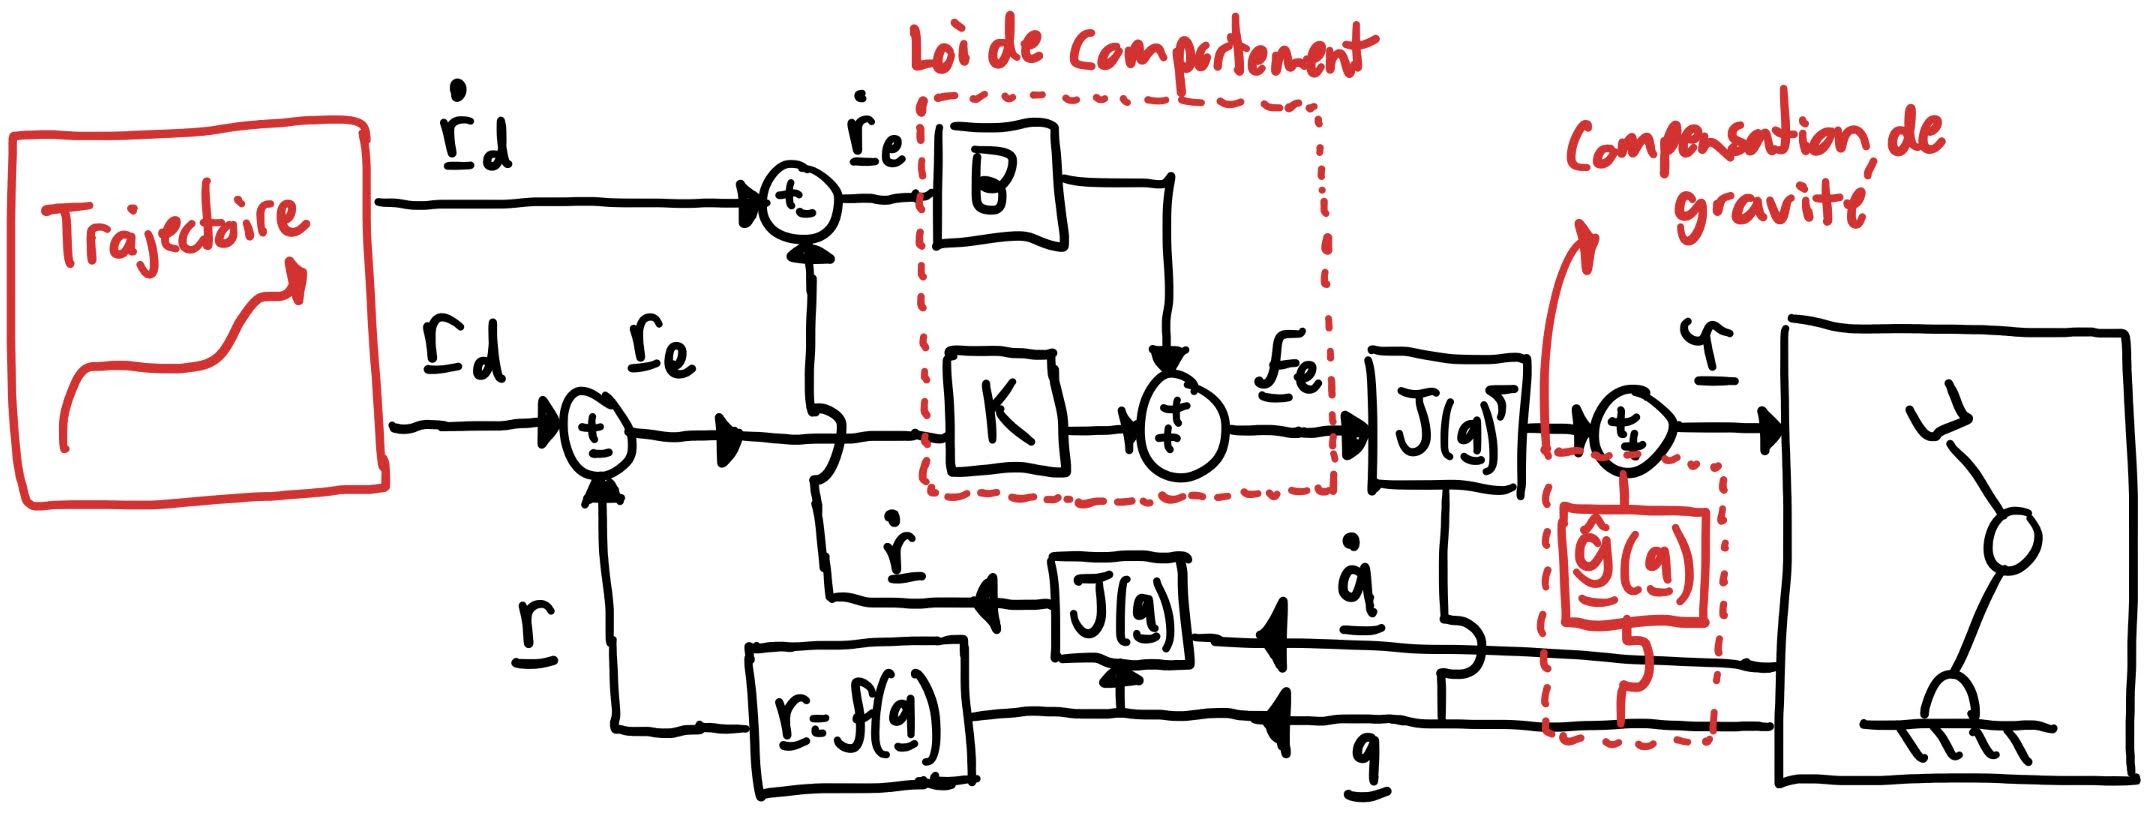
\includegraphics[width=0.99\textwidth]{fig/impedanceeffectorbloc.jpg}
	\caption{Commande de l'impédance de l'effecteur d'un robot : schéma bloc}
	\label{fig:impedanceeffectorbloc}
\end{figure}
%%%%%%%%%%%%%%%%%%%%%%%%%%%%%%%%

\colab{Simulation d'un robot planaire contrôlé en impédance}{https://colab.research.google.com/drive/1EM3hNEwz2aiBqx9GDHoM7QGuPF-Afv1Q?usp=sharing}

\subsection{Équivalence entre une impédance définie aux joints vs. définie à l'effecteur}

Il y a une certaine équivalence locale entre une loi de commande en impédance à l'effecteur et une loi de commande en impédance dans l'espace des joints. Pour un cas simplifié ou la cible $\col{q}_d$ et $\col{r}_d$ sont égale à zéro, les lois de commandes sont données par: 
%%%%%%%%%%%%%%%%%%
\begin{align}
\text{Joints: }
\col{\tau} = - K_q \col{q} - B_q \col{\dot{q}}
\quad\quad
\text{Effecteur: }
\col{\tau} = - J(\col{q})^T   \left[ K_e \col{r} + B_e \col{\dot{r}} \right] 
\end{align}
%%%%%%%%%%%%%%%%%
où on a rajouté les indices $q$ ou $e$ aux matrices pour spécifier l'espace, joint ou effecteur, dans lesquelles elles sont définies. Ensuite si on distribue et utilise la relation de cinématique différentielle, on observe que la matrice d'amortissement $B_e$ à l'effecteur a exactement le même effet qu'une matrice d'amortissement dans l'espace des joints égale à $B_q = J^T B_e J$:
%%%%%%%%%%%%%%%%%%
\begin{align}
\col{\tau} &= - J(\col{q})^T   K_e \col{r} - J(\col{q})^T B_e \col{\dot{r}} \\
\col{\tau} &= - J(\col{q})^T   K_e \col{r} - \underbrace{ [ J(\col{q})^T   B_e  J(\col{q}) ] }_{ B_q } \col{\dot{q}}
\end{align}
%%%%%%%%%%%%%%%%%
Pour des petites variations autour de la position d'équilibre des ressorts virtuels (celle pour laquelle la force nette est nulle), on peut aussi retrouver une équivalence similaire pour la rigidité $K_q = J^T K_e J$:
%%%%%%%%%%%%%%%%%%
\begin{align}
\delta \col{\tau} &= - \underbrace{ [ J(\col{q})^T   K_e  J(\col{q}) ] }_{ K_q }
\delta \col{q} - \underbrace{ [ J(\col{q})^T   B_e  J(\col{q}) ] }_{ B_q }\delta \col{\dot{q}}
\end{align}
%%%%%%%%%%%%%%%%%
Il est à bien noter que ces équivalences sont locales seulement due aux effets non-linéaires. 

%%%%%%%%%%%%%%%%%%%%%%%%%%%%%%%%%%%%%%%%%%%%%%%%%%%%%%%%%%%%%%%%%%%%%%%%%%%%%%%%
\subsection{Convergence des lois de commande en impédance}
\label{sec:impcontrolconvergence}

Pour les robots avec des actionneurs contrôlés en force, une bonne façon de contrôler la position de l'effecteur est d'utiliser l'approche en impédance à l'effecteur avec une matrice $K$ très rigide. C'est l'équivalent de prendre un gros ressort très rigide, attacher une extrémité sur la position cible et l'autre sur l'effecteur du robot. Le robot va être attiré vers la position cible. D'un point de vu énergétique, le robot va converger vers le point ou l'énergie potentielle du système est minimum, ce qui est la position cible si le ressort est la seule source d'énergie potentielle. Pour que le point de convergence soit stable il faut aussi qu'il y ait une certaine forme de dissipation dans le système (qui peut venir des coefficients du ressort virtuel dans $B$ ou bien de phénomènes physique dans les joints du robot) sinon le robot oscillerait autour du point d'énergie potentiel minimum. 
%%%%%%%%%%%%%%%%%%%%%%%%%%%%%%%%
\begin{figure}[h]
	\centering
		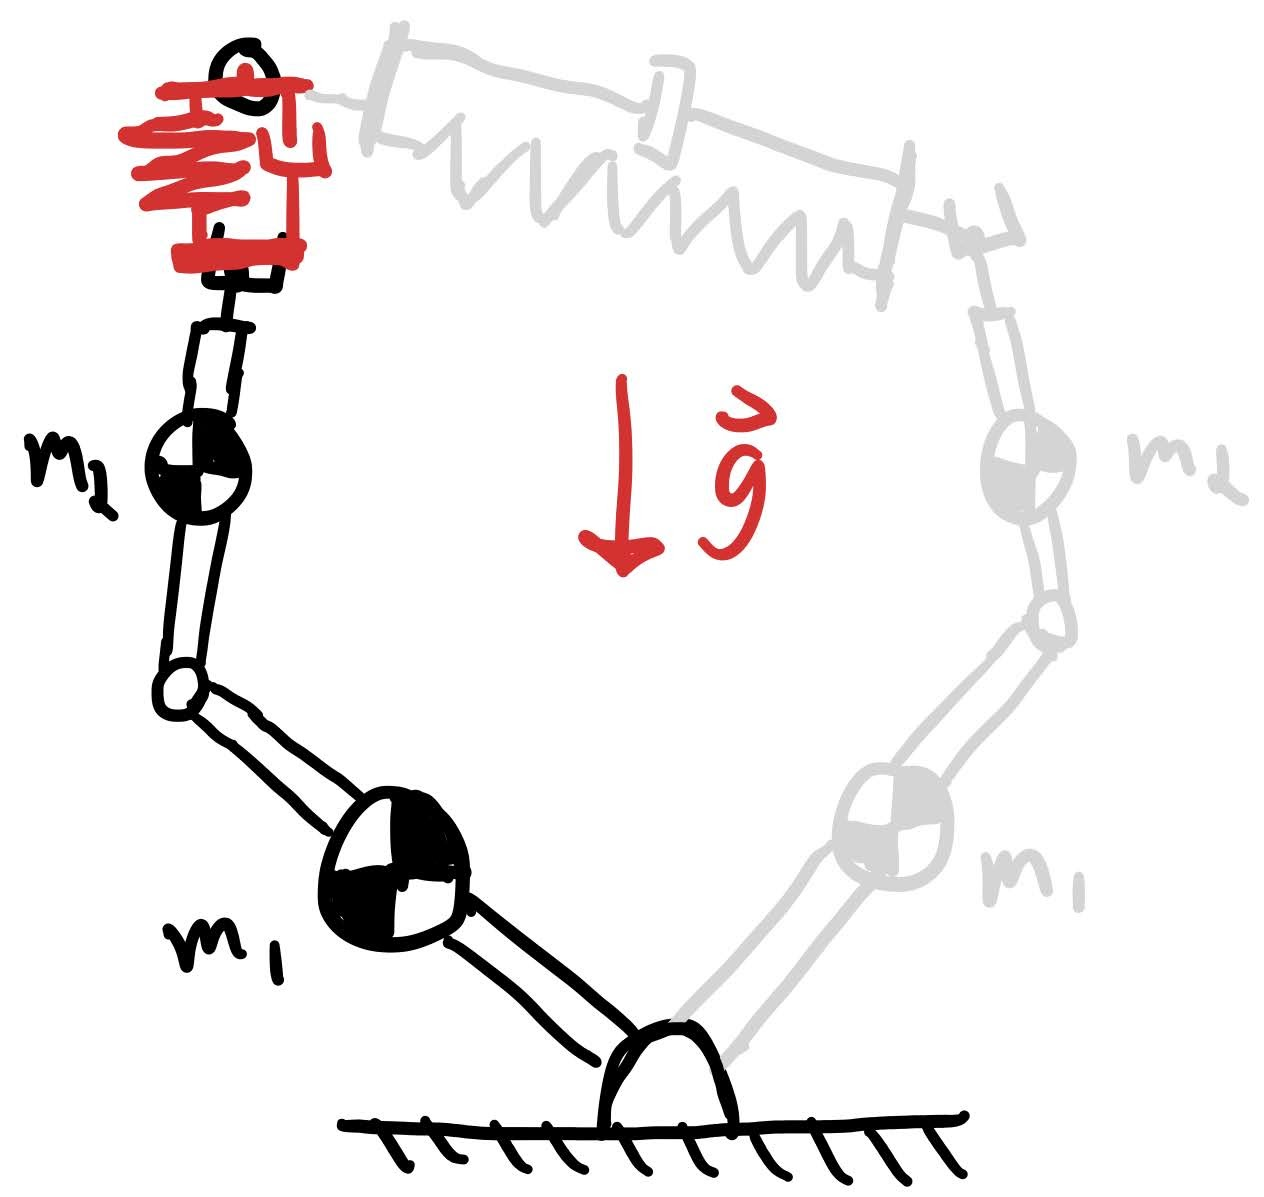
\includegraphics[width=0.5\textwidth]{fig/impedancecontroltaskconvergencegeo.jpg}
	\caption{Convergence d'un contrôleur en impédance à l'effecteur}
	\label{fig:impedancecontroltaskconvergencegeo}
\end{figure}
%%%%%%%%%%%%%%%%%%%%%%%%%%%%%%%%

Comme illustré à la Figure \ref{fig:impedancecontroltaskconvergencegeo}, si considère d'abord le robot comme seulement une chaîne de corps rigide avec leurs propriétés inertielles, on peut bien visualiser qu'un ressort à l'effecteur va attirer le robot sur la cible. Les propriétés inertielles du bras et la géométrie non-linéaire vont influencer la trajectoire, mais dans ce cas le point d'équilibre dépend seulement des forces conservatrice. Si le ressort virtuel de la loi d'impédance est le seul élément qui produit une force conservatrice, alors le point d'équilibre sera la configuration ou l'effecteur est exactement sur la cible. Si le robot est influencé par des forces gravitationnelles, le point d'équilibre sera le point minimum de l'énergie potentielle totale. Le robot aura donc une erreur finale avec une amplitude qui dépend de la force relative du ressort virtuel et de la gravité. Comme illustré à la Figure \ref{fig:impedanceeffectorbloc}, il est toutefois possible d'inclure une \textbf{compensation de gravité} $\col{\hat{g}}$ à une loi de commande en impédance pour éliminer cette erreur finale:
%%%%%%%%%%%%%%%%%%
\begin{align}
\col{\tau} = J(\col{q})^T   \left[ K \col{r}_e + B \col{\dot{r}}_e \right] + \col{\hat{g}}(\col{q})
\end{align} 
%%%%%%%%%%%%%%%%%
où $\col{\hat{g}}$ est l'estimation par le contrôleur (basé sur un modèle) du vecteur des forces gravitationnelles dans l'espace des joints. Finalement, un autre phénomène courant qui pourrait causer une erreur final serait s'il y a de la friction sèche dans les joints du robot. Le robot pourrait rester pris à un point ou la force commandée est égale à la friction sèche dans le système.

Cette analyse qualitative basée sur des principes énergétiques peut être formalisé avec une analyse de la stabilité avec la méthode de \textit{Lyapunov}. Si on considère les équations génériques de la dynamique du robot manipulateur avec des actionneurs contrôlés en forces:
%%%%%%%%%%%%%%%%%%
\begin{align}
\underbrace{
H \ddot{\col{q}} + C \dot{\col{q}} 
}_{\text{Forces inertielles }}
+ 
\underbrace{
\col{d}
}_{\text{Forces dissipatives }}
+ 
\underbrace{
\col{g} 
}_{\text{Forces conservatrices }}
= \col{\tau}
\end{align}
%%%%%%%%%%%%%%%%%
avec comme loi de commande, une impédance à l'effecteur incluant une compensation de gravité:
%%%%%%%%%%%%%%%%%%
\begin{align}
\col{\tau} = J^T   \left[ K \col{r}_e + B \col{\dot{r}}_e \right] + \col{\hat{g}}
\end{align}
%%%%%%%%%%%%%%%%%
En utilisant comme fonction candidate de \textit{Lyapunov} l'énergie mécanique réelle plus l'énergie potentielle virtuelle dans le ressort du contrôleur:
%%%%%%%%%%%%%%%%%%
\begin{align}
V = 
\underbrace{
1/2 \, \dot{\col{q}}^T H \dot{\col{q}} 
}_{\text{ Énergie cinétique réelle du robot }}
+
\underbrace{
1/2 \, \col{r}_e^T K \col{r}_e
}_{\text{ Énergie potentielle virtuelle du ressort }}
\end{align}
%%%%%%%%%%%%%%%%%
Il est possible de démontré que cette fonction est toujours décroissante dans le temps sous certaines conditions:
%%%%%%%%%%%%%%%%%%
\begin{align}
\dot{V} &= \frac{d}{dt} \left[ 1/2 \,  \dot{\col{q}}^T H \dot{\col{q}}  + 1/2 \, \col{r}_e^T K \col{r}_e \right]  \\
\dot{V} &= \dot{\col{q}}^T 
\left[ 
H \ddot{\col{q}} + 2 \dot{H} \dot{\col{q}}
\right] +
\col{r}_e^T K \col{\dot{r}}_e
\\%%%%%%%%%%%%%
\dot{V} &= \dot{\col{q}}^T 
\left[ 
\col{\tau} - \col{g} - \col{d}
\right] -
\col{\dot{r}}^T K \col{r}_e
\quad \quad
\text{pour une position désirée fixe: }  \col{\dot{r}}_e = \col{\dot{r}}_d - \col{\dot{r}} = - \col{\dot{r}}
\\%%%%%%%%%%%%%
\dot{V} &= \dot{\col{q}}^T 
\left[ 
\col{\tau} - \col{g} - \col{d}
\right] -
\col{\dot{q}}^T J^T K \col{r}_e
\\%%%%%%%%%%%%%
\dot{V} &= \dot{\col{q}}^T 
\left[ 
\col{\tau} - \col{g} - \col{d}
\right] -
\col{\dot{q}}^T J^T K \col{r}_e
\\%%%%%%%%%%%%%
\dot{V} &= \dot{\col{q}}^T 
\left[ 
\col{\tau} - \col{g} - \col{d}
- J^T K \col{r}_e
\right]
\\%%%%%%%%%%%%%
\dot{V} &= \dot{\col{q}}^T 
\left[ 
J^T   \left[ K \col{r}_e + B \col{\dot{r}}_e \right] + \col{\hat{g}}
- \col{g} - \col{d}
- J^T K \col{r}_e
\right]
\\%%%%%%%%%%%%%
\dot{V} &= \dot{\col{q}}^T 
\left[ 
J^T  K \col{r}_e 
- J^T B \col{\dot{r}}
+ \col{\hat{g}}
- \col{g} - \col{d}
- J^T K \col{r}_e
\right]
\\%%%%%%%%%%%%%
\dot{V} &= \dot{\col{q}}^T 
\left[ 
- J^T B J \col{\dot{q}}
+ \col{\hat{g}}
- \col{g} - \col{d}
\right]
\\%%%%%%%%%%%%%
\dot{V} &= \dot{\col{q}}^T 
\left[ 
- J^T B J \col{\dot{q}} - \col{d}
\right]
\quad \quad
\text{si la compensation de gravité est parfaite}
\\%%%%%%%%%%%%%
\dot{V} &= \dot{\col{q}}^T 
\left[ 
- J^T B J \col{\dot{q}} - D \col{\dot{q}}
\right]
\quad \quad
\text{si on considère la friction dans les joints du robot comme linéaire}
\\%%%%%%%%%%%%%
\dot{V} &= - \dot{\col{q}}^T 
\left[ 
J^T B J + D 
\right] \col{\dot{q}}
\\%%%%%%%%%%%%%
\dot{V} &< 0 \quad  
\forall \col{\dot{q}} \neq \col{0} \quad 
\text{si} \left[ J^T B J + D \right]  > 0
\quad\quad \Rightarrow \quad\quad
\lim_{t \rightarrow \infty} \col{r}_e(t) = \col{0} \quad \& \quad
\lim_{t \rightarrow \infty} \col{\dot{q}}(t) = \col{0}
\end{align} 
%%%%%%%%%%%%%%%%%
Ce qui démontre que le système va nécessairement converger vers le point minimum de la fonction $V$, ce qui correspond à $\col{q} = \col{0}$ et $\col{r}_e = \col{0}$, avec comme condition que les termes d'amortissement total du système (contrôleur + friction naturelle) sont positifs. Cette analyse peut aussi être faites pour une impédance dans le domaine des joints, et une combinaison des deux, pour obtenir des conclusions équivalentes. 

% %%%%%%%%%%%%%%%%%%%%%%%%%%%%%%%%
% \begin{figure}[th]
% 	\centering
% 		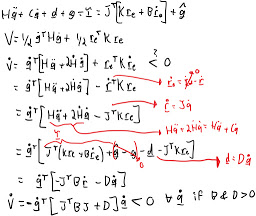
\includegraphics[width=0.70\textwidth]{fig/impedancecontroltaskconvergencemath.jpg}
% 	\caption{Contrôleur en impédance à l'effecteur: analyse de convergence}
% 	\label{fig:impedancecontroltaskconvergencemath}
% \end{figure}
% ¢


%%%%%%%%%%%%%%%%%%%%%%%%%%%%%%%%%%%%%%%%%%%%%%
\section{Commande en admittance}
\label{sec:admcontrol}

Pour un contrôle en admittance, dans l'espace des joints ou de la tâche, des capteurs mesurent des forces et le déplacement du robot est contrôlé à bas niveau, soit en position ou en vitesse. Si les actionneurs sont asservis en position, la relation générique est:
%%%%%%%%%%%%%%%%%%
\begin{align}
q_i = \frac{1}{Z_i(s)} \tau_i
\label{eq:admipos}
\end{align}
%%%%%%%%%%%%%%%%%
où $q_i$ est une consigne de position pour le joint $i$, $Z_i$ est une impédance désirée pour le joint $i$ et $\tau_i$ est la force mesurée au joint $i$.
Si les actionneurs sont asservis en vitesse à bas niveau, la relation générique est:
%%%%%%%%%%%%%%%%%%
\begin{align}
\dot{q}_i = \frac{s}{Z_i(s)} \tau_i
\label{eq:admispeed}
\end{align}
%%%%%%%%%%%%%%%%%

Lorsqu'on implémente une loi de commande il est préférable d'éviter de dériver des signaux, donc certaines combinaison de type de consigne bas-niveau (position vs. vitesse) avec un type d'impédance sont préférable. Par exemple, pour émuler une force proportionnelle à une vitesse $Z_i(s) = b_i s$ avec des actionneurs contrôlés en vitesse, l'équation \eqref{eq:admispeed} se réduit à 
%%%%%%%%%%%%%%%%%%
\begin{align}
\dot{q}_i = \frac{1}{b} \tau_i
\end{align}
%%%%%%%%%%%%%%%%%
donc simplement une relation algébrique entre les signaux. Avec des actionneurs contrôlés en position l'équation \eqref{eq:admipos} se réduit à 
%%%%%%%%%%%%%%%%%%
\begin{align}
q_i = \frac{1}{b s} \tau_i = \frac{1}{b} \int \tau_i
\end{align}
%%%%%%%%%%%%%%%%%
ce qui implique d'intégrer le signal de force. Par contre, si on désire émuler un système masse-ressort-amortisseur c'est l'approche avec des actionneurs en position qui est préférable. Avec des actionneurs contrôlés en position l'équation \eqref{eq:admipos} se réduit dans ce cas à  
%%%%%%%%%%%%%%%%%%
\begin{align}
\dot{q}_i = \frac{1}{ms^2+bs+k} \tau_i
\end{align}
%%%%%%%%%%%%%%%%%
La fonction de transfert a deux pôles donc l'implémentation inclurait deux intégrales. Avec des actionneurs contrôlés en vitesse l'équation \eqref{eq:admispeed} se réduit dans ce cas à 
%%%%%%%%%%%%%%%%%%
\begin{align}
\dot{q}_i = \frac{s}{ms^2+bs+k} \tau_i
\end{align}
%%%%%%%%%%%%%%%%%
une fonction de transfert qui a en plus un zéro, donc demanderait de dériver un signal en plus des deux intégrales. Pour l'implémentation d'une loi de commande, l'idéal lorsque possible est une relation algébrique. Si on doit avoir une relation différentielle il est préférable d'avoir seulement des intégrales. Les opérations de dérivations sont à éviter. 

\subsection{Commande en admittance aux joints}
\label{sec:jointadmcontrol}

Pour un contrôle en admittance dans l'espace des joints, des capteurs de forces vont mesurée la force actuelle à chaque joint et commander un déplacement à l'actionneur relié. Les lois en admittance peuvent aussi être exprimées en format matricielle pour décrire le comportement de tous les joints en une seule équation. La Figure \ref{fig:admitancecontroljointspace1} présente un contrôleur en admittance de type amortisseurs avec comme comportement cible la relation:
%%%%%%%%%%%%%%%%%%
\begin{align}
B \col{\dot{q}} = \col{\tau}
\end{align}
%%%%%%%%%%%%%%%%%
pour un robot contrôlé en vitesse à bas niveau dans l'espace des joints, avec des capteurs qui mesure le couple de chaque joint. 
%%%%%%%%%%%%%%%%%%%%%%%%%%%%%%%%
\begin{figure}[th]
	\centering
		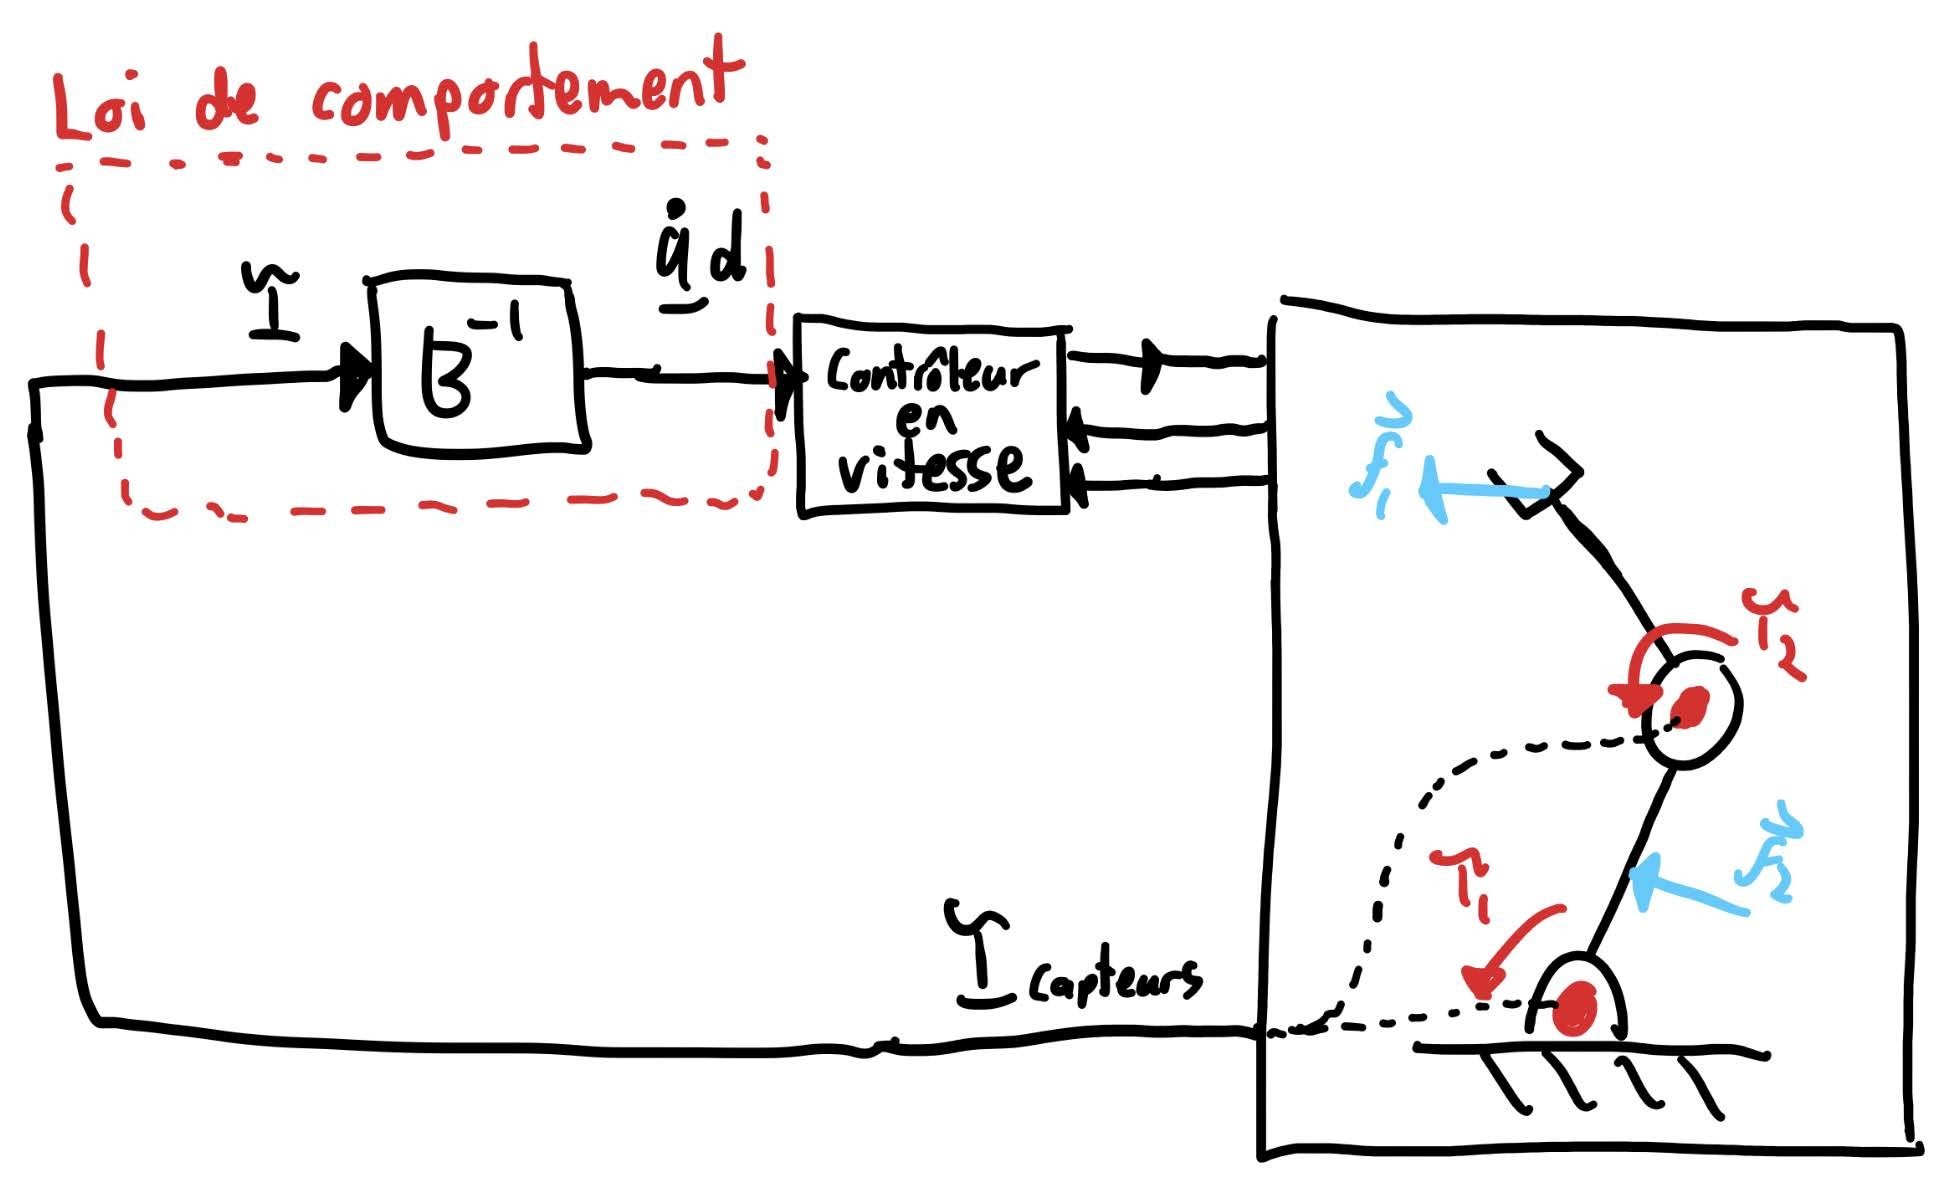
\includegraphics[width=0.70\textwidth]{fig/admitancecontroljointspace1.jpg}
	\caption{Commande de l'admittance au joints d'un robot : schéma bloc}
	\label{fig:admitancecontroljointspace1}
\end{figure}
%%%%%%%%%%%%%%%%%%%%%%%%%%%%%%%%

La Figure \ref{fig:admitancecontroljointspace} présente le schéma bloc d'un contrôleur en admittance avec comme comportement cible la relation:
%%%%%%%%%%%%%%%%%%
\begin{align}
M \col{\ddot{q}} + B \col{\dot{q}} + K \col{q} = \col{\tau}
\end{align}
%%%%%%%%%%%%%%%%%
pour un robot contrôlé en position à bas niveau dans l'espace des joints, avec des capteurs qui mesure le couple de chaque joint. Pour ce cas il y a deux intégrale dans la loi de commande. On peut interpréter le bloc "loi de comportement" à la Figure \ref{fig:admitancecontroljointspace} qui est tout simplement la simulation d'un système masse-ressort-amortisseur qui reçoit en entrée une force réelle lue par un capteur. Le résultat de la simulation est ensuite envoyer à un contrôleur en déplacement. Le robot va donc émuler le système virtuel simulé. 
%%%%%%%%%%%%%%%%%%%%%%%%%%%%%%%%
\begin{figure}[h]
	\centering
		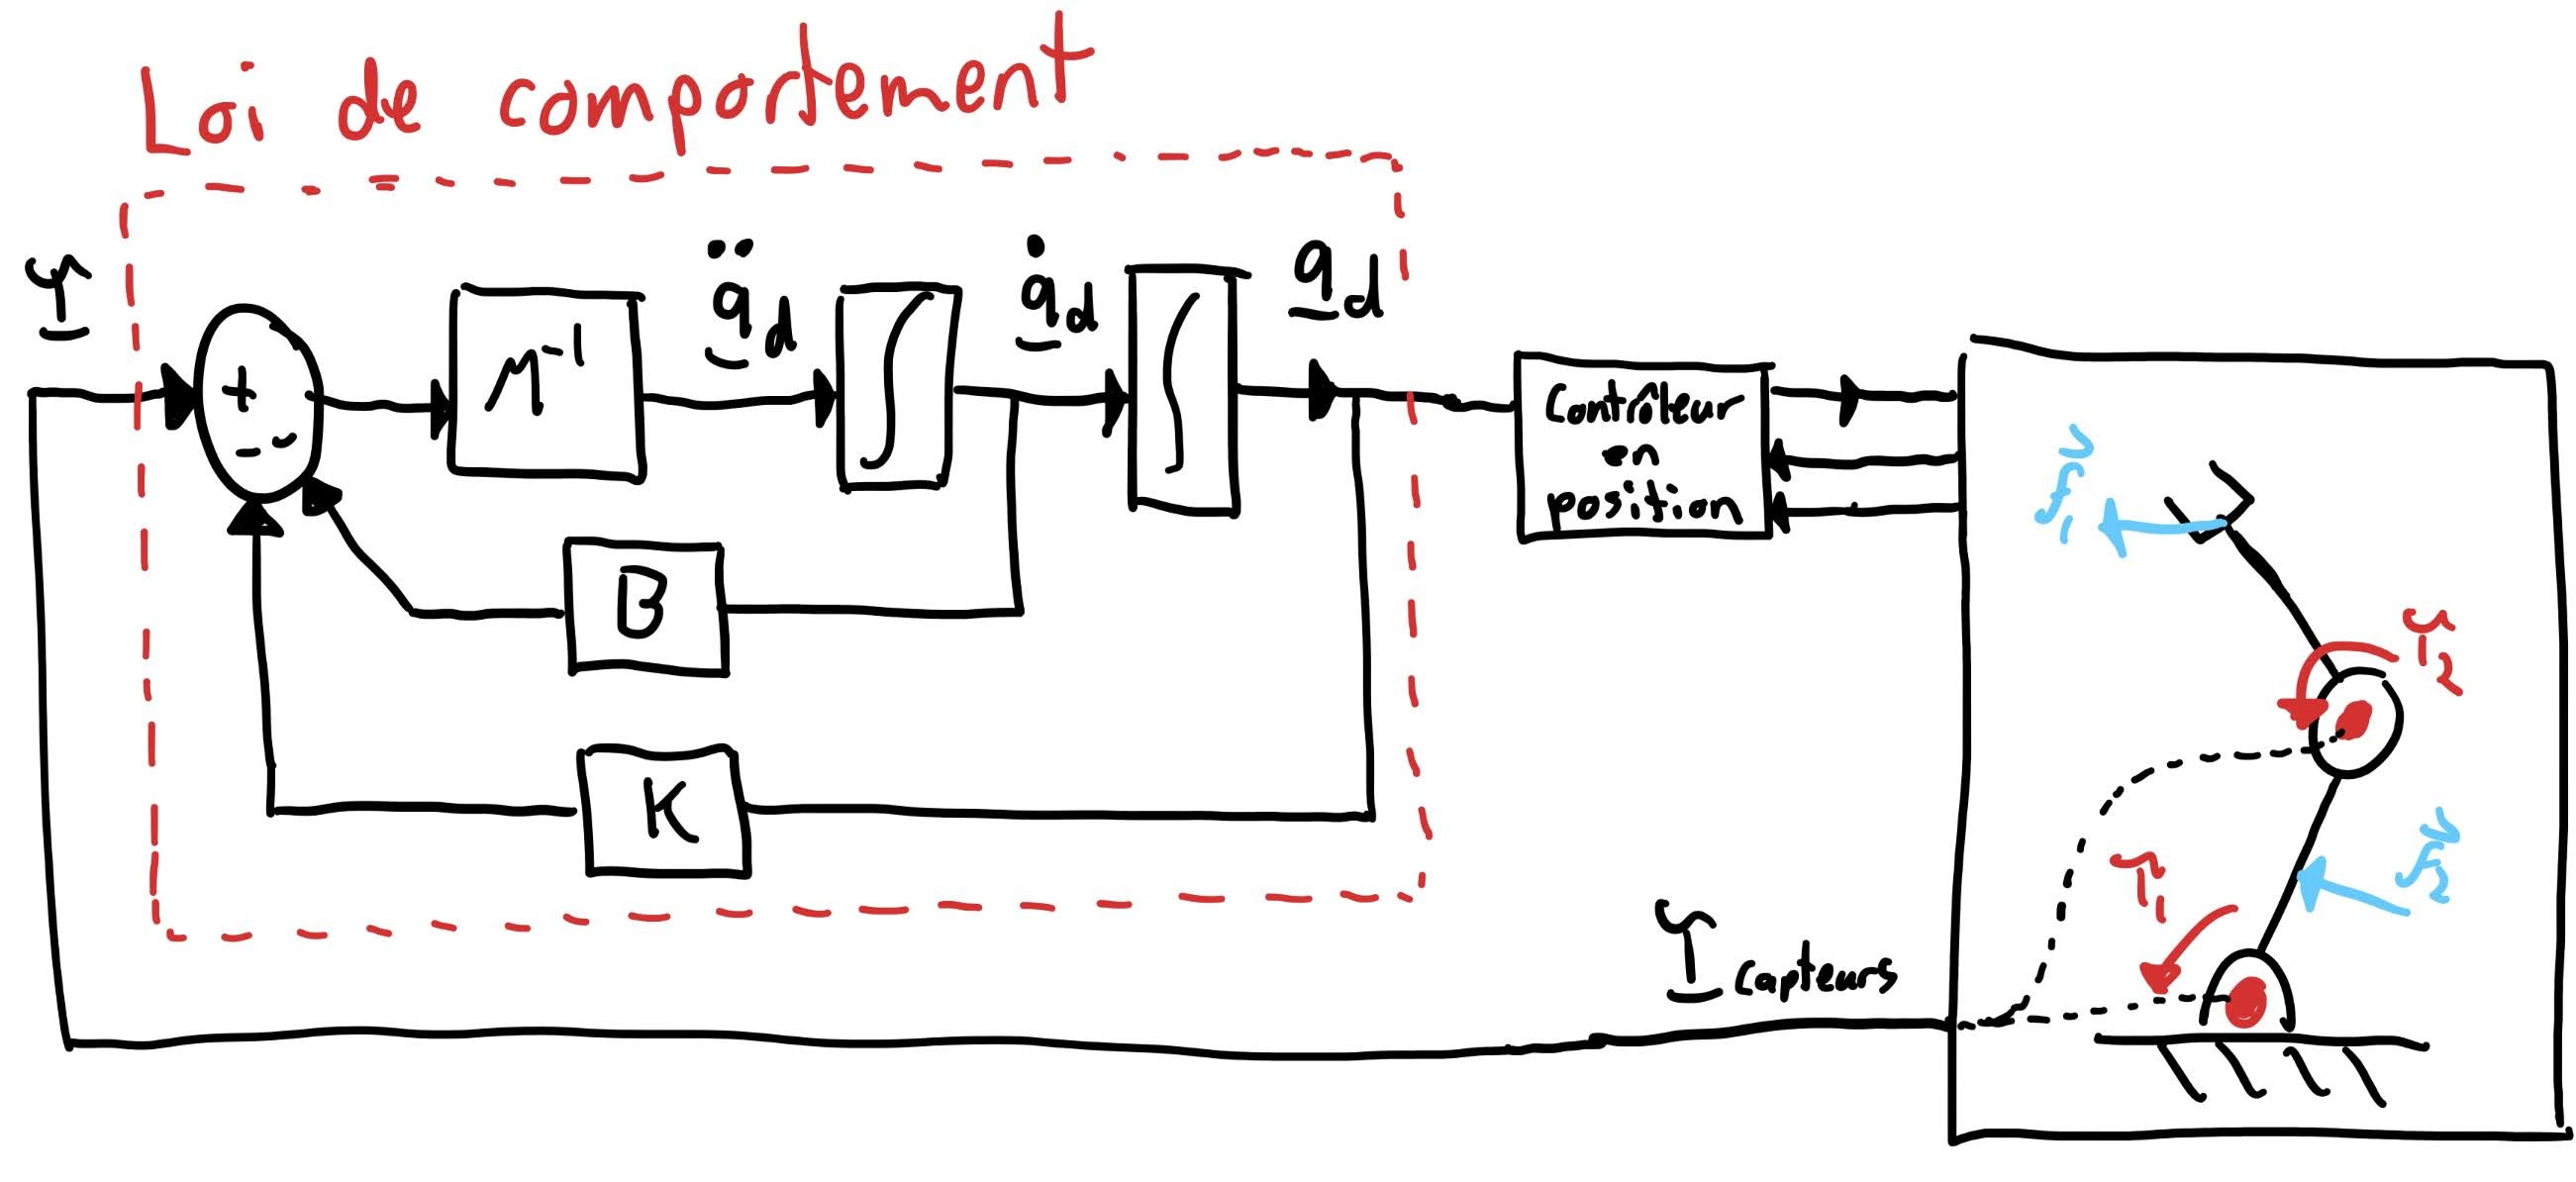
\includegraphics[width=0.85\textwidth]{fig/admitancecontroljointspace.jpg}
	\caption{Commande de l'admittance au joints d'un robot : schéma bloc}
	\label{fig:admitancecontroljointspace}
\end{figure}
%%%%%%%%%%%%%%%%%%%%%%%%%%%%%%%%

\video{Commande en admittance d'un robot manipulateur}{https://youtu.be/SP5bISWmkT0}

\subsection{Commande en admittance de l'effecteur}
\label{sec:effadmcontrol}

L'approche en admittance dans l'espace de l'effecteur est basée sur une mesure de la force à l'effecteur (généralement avec une cellule de charge) et le contrôle du déplacement de l'effecteur à bas niveau. La Figure \ref{fig:admittancecontroltaskspace1} présente un schéma bloc d'une loi de commande en admittance pour imposer un comportement: %%%%%%%%%%%%%%%%%%
\begin{align}
B \col{\dot{r}} = \col{f}_e
\end{align}
%%%%%%%%%%%%%%%%%
Une chose à noter est que généralement la cellule de charge va mesurer les composantes du vecteur force $\Vec{f}_e$ dans une base vectorielle mobile $t$ attachée à l'outil. Il faut donc faire un changement de base avec la matrice de rotation ${}^{w}R^t$ pour avoir les composantes dans la base vectorielle fixe $w$ dans laquelle le reste des autres vecteurs sont exprimés. La matrice de rotation ${}^{w}R^t$ doit donc être obtenue basé sur la positon des joints actuels en utilisant la relation de cinématique directe pour l'orientation. La loi de commande de la Figure \ref{fig:admittancecontroltaskspace1} est utilisée pour le mode démonstration (\textit{teach mode}) des robots manipulateur, i.e. le mode ou un opérateur peut déplacer le robot manuellement dans l'espace. Avec cette loi de commande, un humain peut pousser sur l'effecteur du robot et le robot se déplacera alors dans le sens de la poussée avec une vitesse proportionnelle à l'amplitude de la poussée. Si il n'y a aucune poussée le robot reste en place. 
%%%%%%%%%%%%%%%%%%%%%%%%%%%%%%%%
\begin{figure}[h]
	\centering
		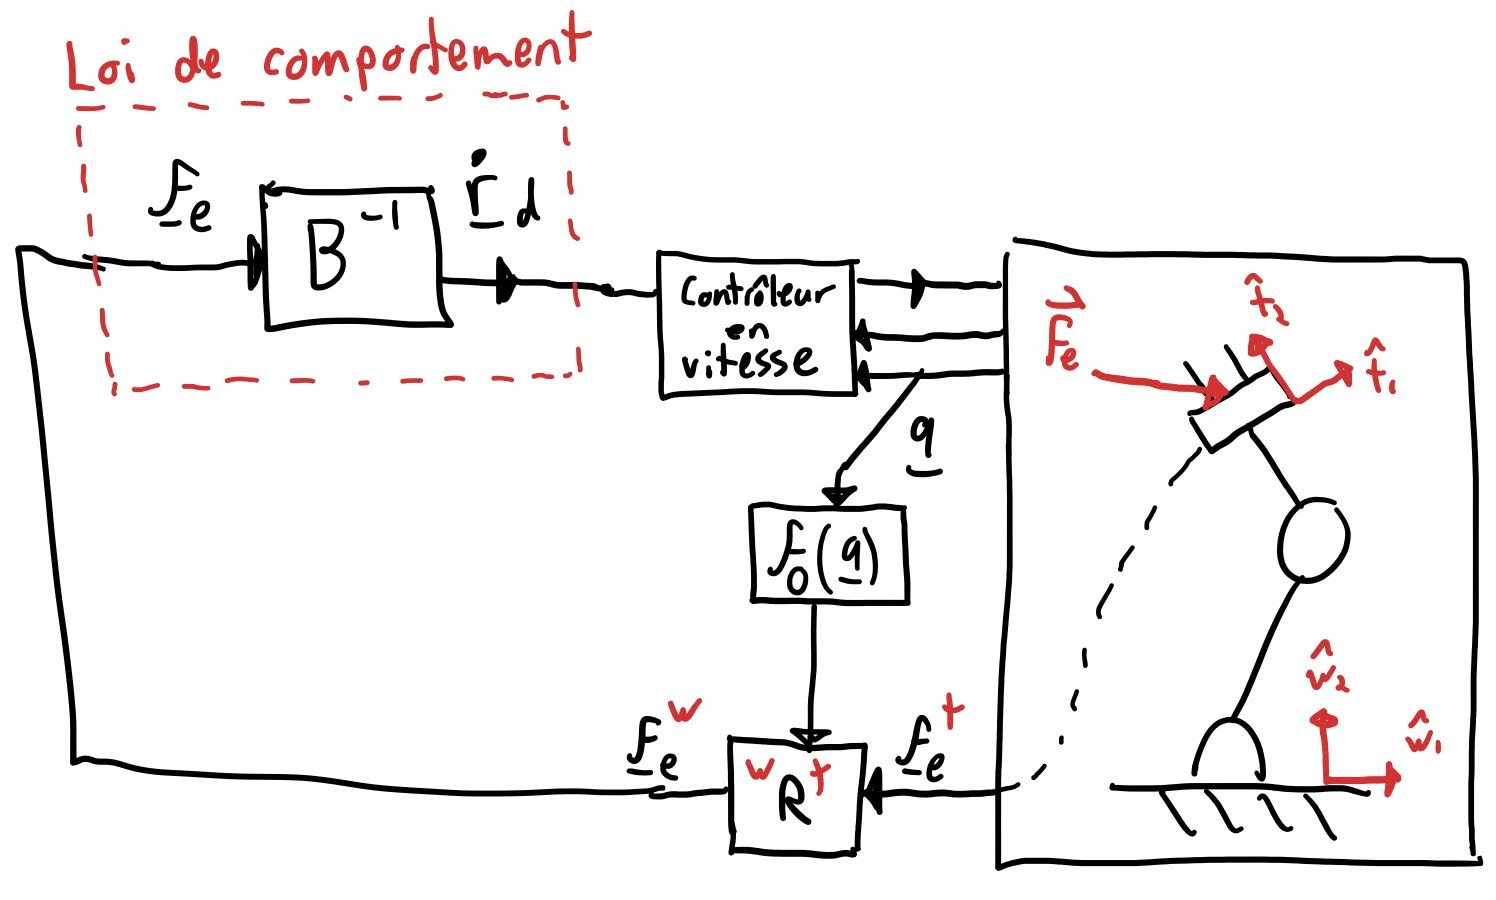
\includegraphics[width=0.80\textwidth]{fig/admittancecontroltaskspace1.jpg}
	\caption{Commande de l'admittance à l'effecteur d'un robot avec une loi de comportement de type amortisseur: schéma bloc}
	\label{fig:admittancecontroltaskspace1}
\end{figure}
%%%%%%%%%%%%%%%%%%%%%%%%%%%%%%%%

La Figure \ref{fig:admittancecontroltaskspace1} montre le schéma bloc d'une loi de commande plus générique pour une loi de comportement égale à une masse-ressort-amortisseur à l'effecteur:
%%%%%%%%%%%%%%%%%%
\begin{align}
M \col{\ddot{r}} + B \col{\dot{r}} + K \col{r}= \col{f}_e
\end{align}
%%%%%%%%%%%%%%%%%
%%%%%%%%%%%%%%%%%%%%%%%%%%%%%%%%
\begin{figure}[h]
	\centering
		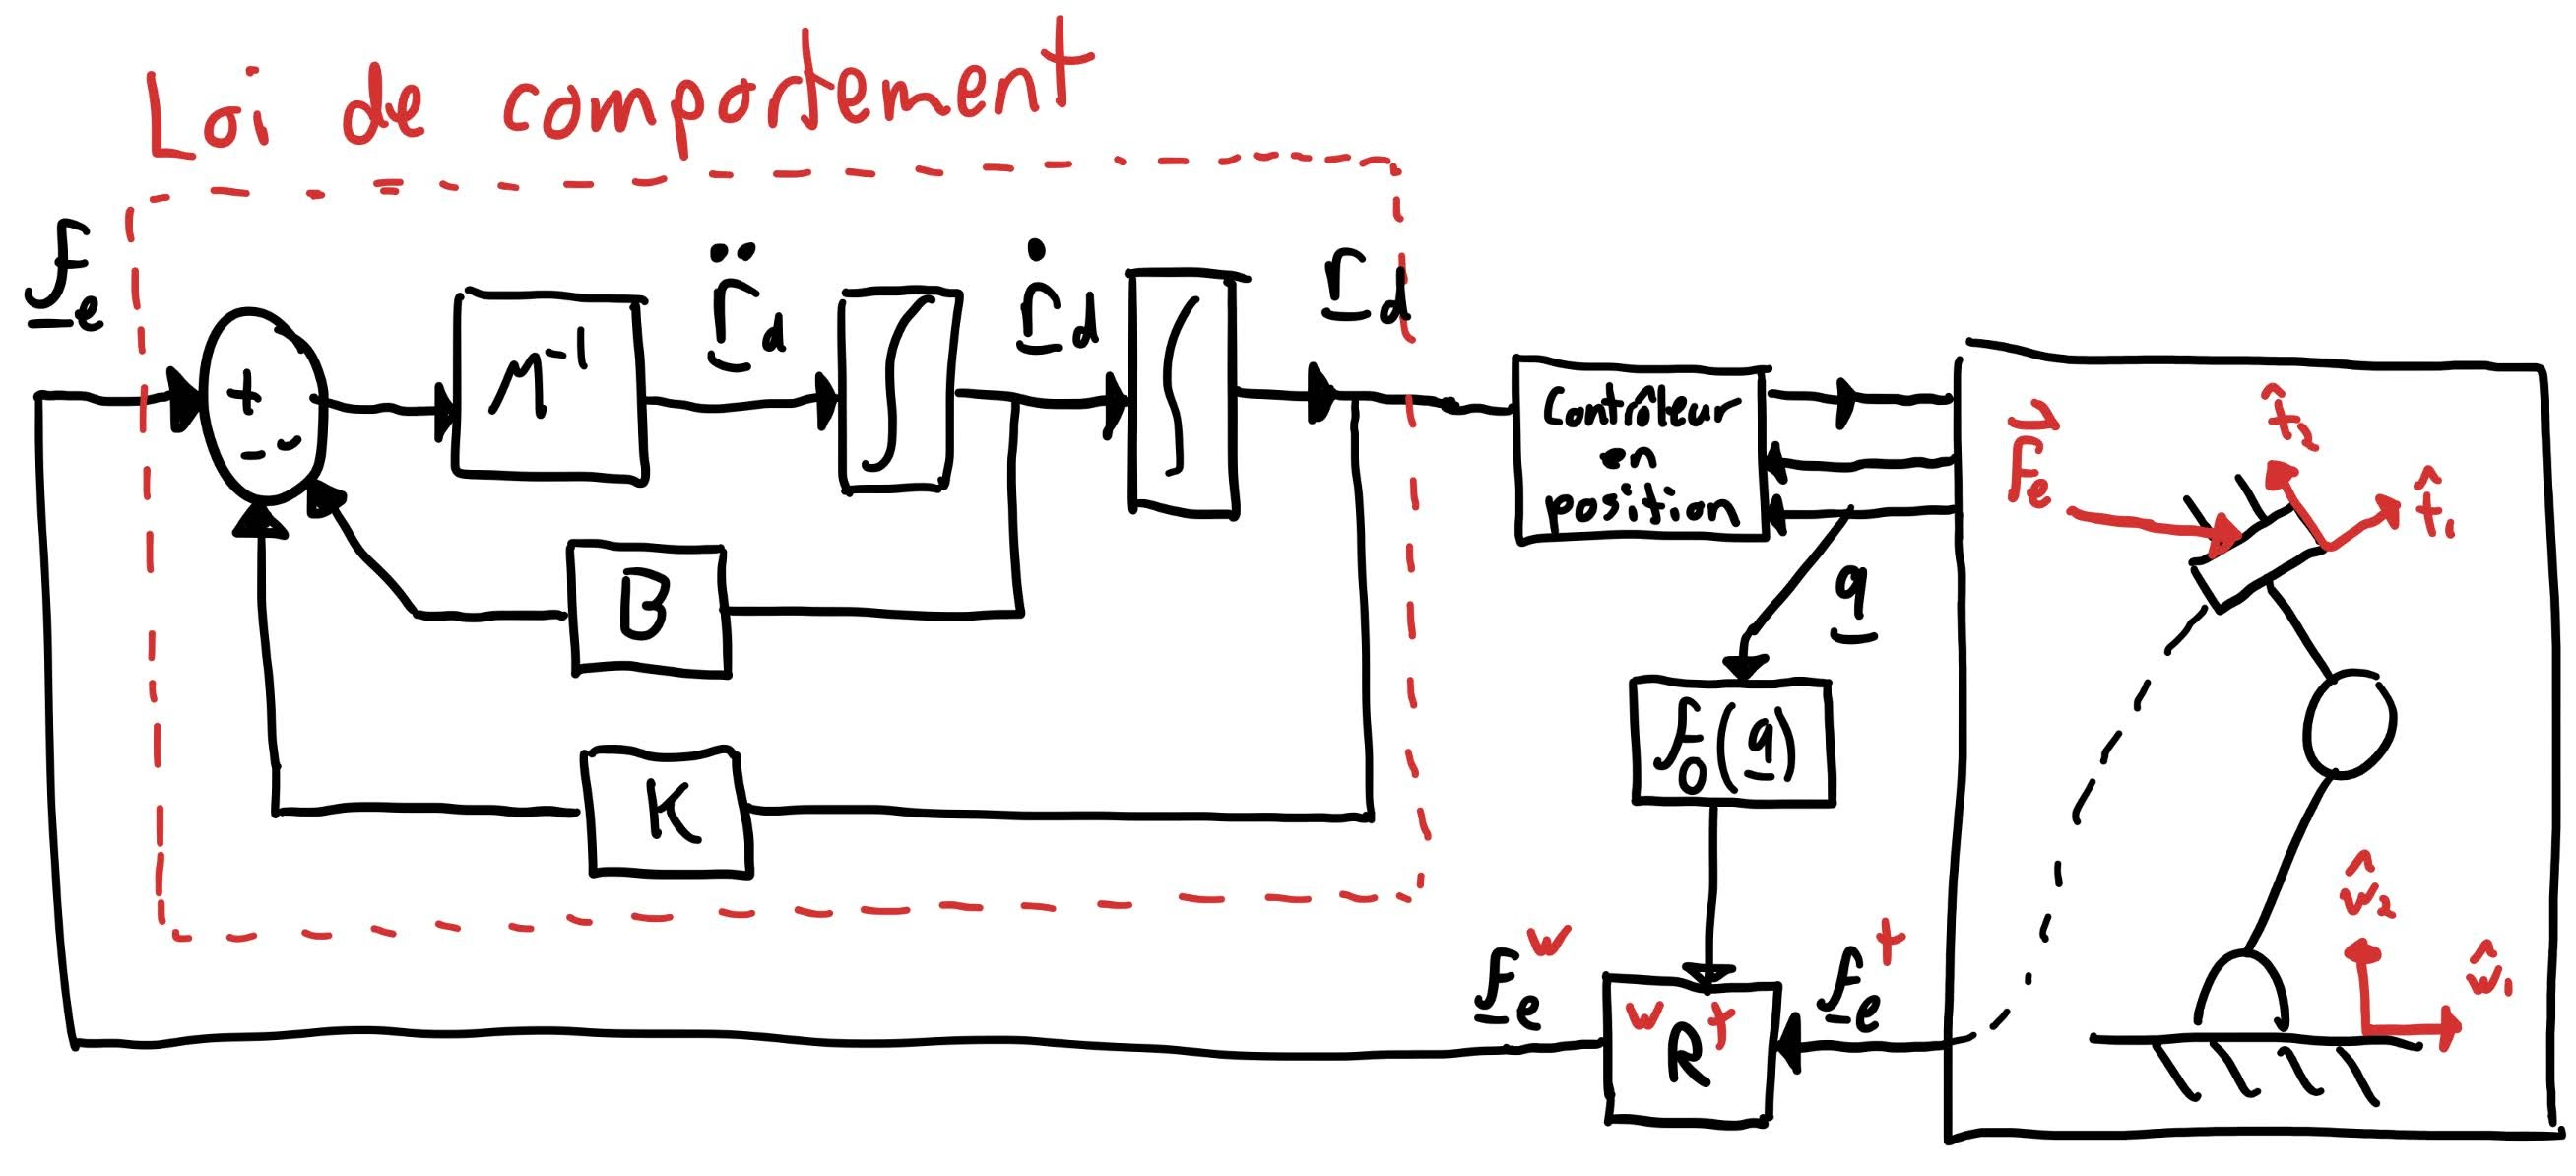
\includegraphics[width=0.99\textwidth]{fig/admittancecontroltaskspace.jpg}
	\caption{Commande de l'admittance à l'effecteur d'un robot avec une loi de comportement de type masse-ressort-amortisseur: schéma bloc}
	\label{fig:admittancecontroltaskspace}
\end{figure}
%%%%%%%%%%%%%%%%%%%%%%%%%%%%%%%%
Il est à noté que les Figures \ref{fig:admittancecontroltaskspace1} et \ref{fig:admittancecontroltaskspace} ne montre pas le détail de la boucle interne du contrôleur en vitesse ou position de l'effecteur. Les méthodes présentées aux sections \ref{sec:speedcontrol} et \ref{sec:positioncontrol} peuvent être utilisée. Une différence à noter pour l'approche en admittance basée sur l'utilisation d'une cellule de charge à l'effecteur du robot, par rapport aux autres approches présentés est que seul les forces qui sont appliquées à l'effecteur (en aval de la cellule de charge) vont influencer la position du robot. Si une force est appliqué sur les liens du robot en amont de la cellule de charge, le contrôleur n'aura pas connaissance de cette force externe qui ne sera donc pas pris en compte dans le calcul du déplacement du robot basée sur la loi de comportement désirée.


